\chapter{Experimentación}
En esta sección explicamos los experimentos realizados para construir un generador y un clasificador de imágenes que funcionen adecuadamente. Para ambos productos realizamos varios experimentos, comprobando que configuración funciona mejor en cada uno de ellos.

\section{Generación de imágenes sintéticas}
La generación de imágenes la vamos a realizar utilizando el modelo desarrollado por Esser et al. \cite{esser2021taming}, descrito en la revisión del estado del arte de este TFG. Vamos a intentar generar imágenes de moléculas organometálicas, para ello entrenaremos el modelo sobre las imágenes positivas del conjunto de datos sin aplicarles \textit{data augmentation} y haremos lo mismo aplicando \textit{data augmentation} 1, \textit{data augmentation} 2 y \textit{data augmentation} 3. En estos tres últimos casos, el número de imágenes utilizado para entrenar se multiplica por 4, ya que aplicamos las secuencias de transformaciones 3 veces. 

Sobre los cuatro conjuntos de datos se entrenarán modelos con diferente número de épocas, desde 70 hasta 170, aumentando de 20 en 20. De esta forma tendremos $4 * |[70, 90, 110, 130, 150, 170]| = 4 * 6 = 24$ modelos diferentes.

Una vez entrenados los modelos, probamos a generar imágenes a partir de estos para ver cuál se comporta mejor. Para ello, debemos introducirles algún tipo de imagen de entrada. 

En las páginas siguientes se muestran los resultados. Cada fila corresponde a una imagen de entrada al modelo. En las columnas, la primera muestra la imagen de entrada mientras que cada una de las siguientes corresponde con un modelo entrenado durante x épocas, desde 70 hasta 170 (70, 90, 110, 130, 150, 170).

Se puede observar como la versión sin \textit{data augmentation} no funciona bien, produce imágenes sin apenas estructura. Esto se debe a que sólo se utilizan 162 imágenes, cifra muy baja para una arquitectura de deep learning como es un Transformer. Con \textit{data augmentation} 1 tampoco se observan resultados de buena calidad, puede que algo mejores que en el caso anterior pero sin muchas diferencias.

Es en \textit{data augmentation} 2 cuando ya se empiezan a ver mayores diferencias. El uso de transformaciones más fuertes crea un conjunto heterogéneo de imágenes y el modelo puede aprender más características de estas. Los resultados son aceptables, aunque el cambio de color que las transformaciones producían en algunas imágenes de entrenamiento ha dado lugar a fondos grisáceos en sus homólogas sintéticas. 

Con el tercer \textit{data augmentation} estos fondos grisáceos son mucho más marcados. Recordamos que estas transformaciones eran mucho más fuertes, por lo que se traslada a las imágenes sintéticas.


\begin{figure}[H]
\centering
    \caption{Resultados de entrenar los modelos sobre el conjunto de datos sin \textit{data augmentation}. La primera columna representa la imagen de entrada, el resto los diferentes modelos entrenados desde 70 hasta 170 épocas, tomadas de 20 en 20.} 
    \fbox{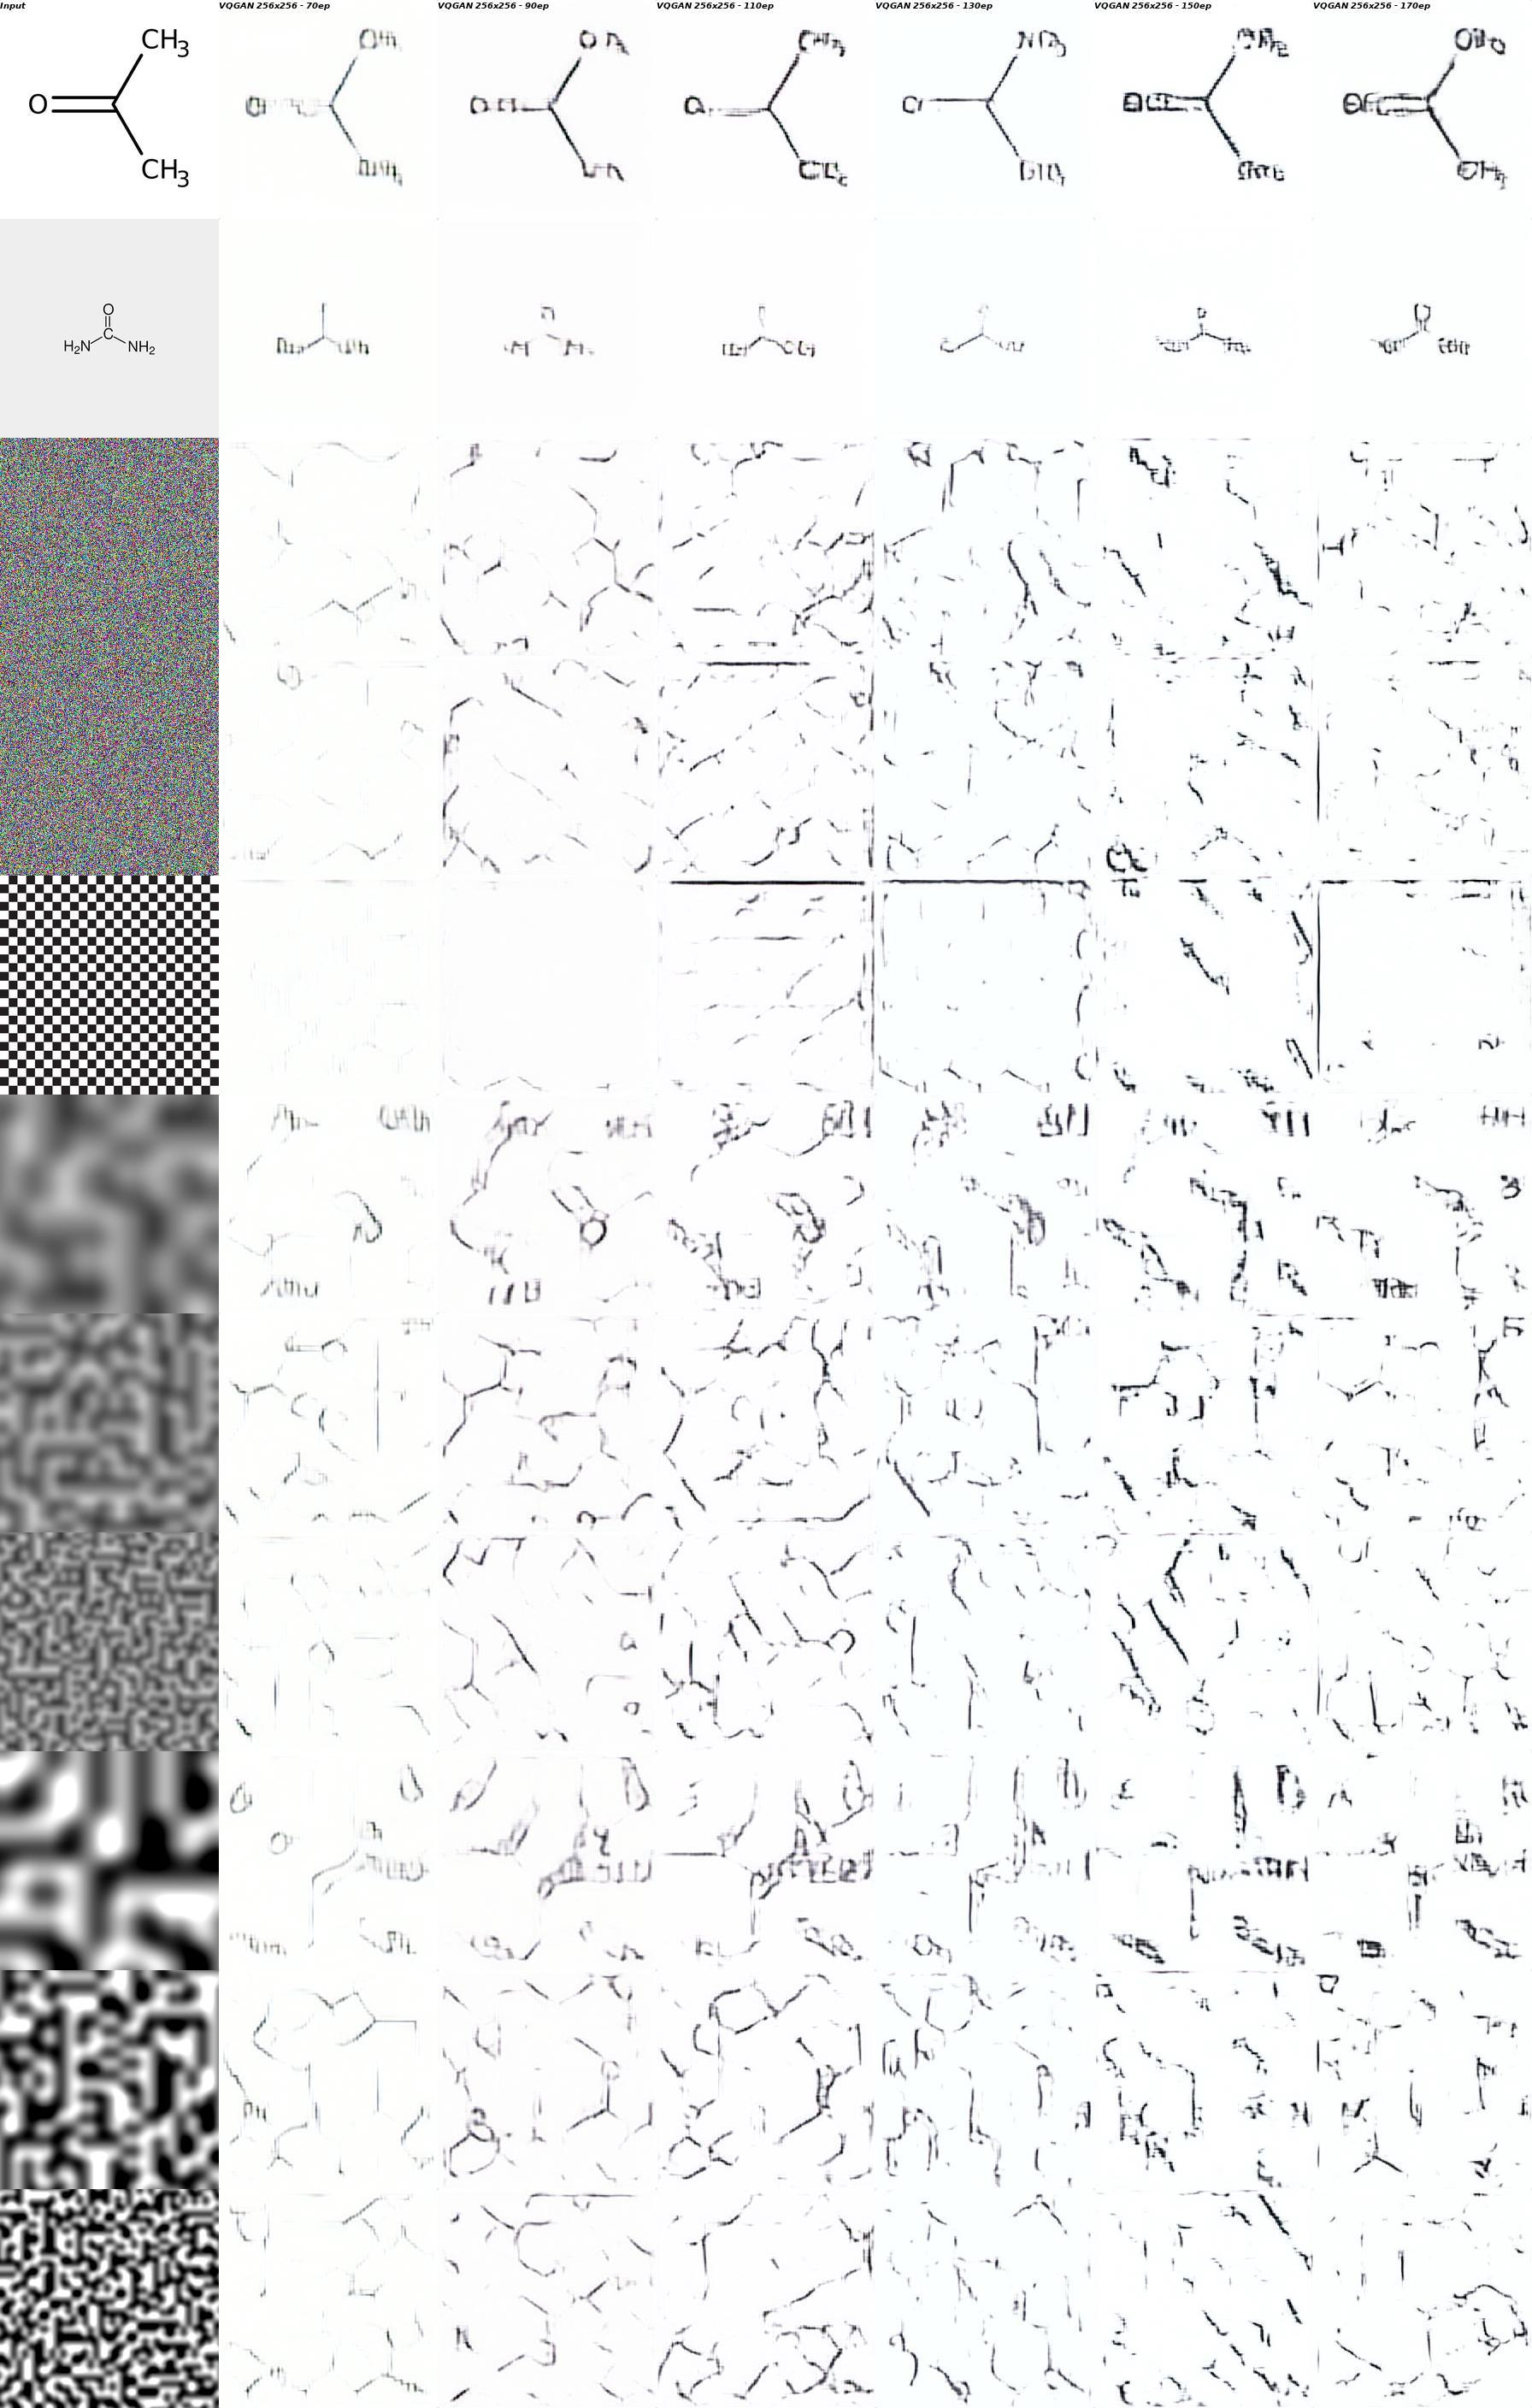
\includegraphics[scale=0.2]{imagenes/image_generation/256/256_1.jpg}}  
\end{figure}

\begin{figure}[H]
\centering
    \fbox{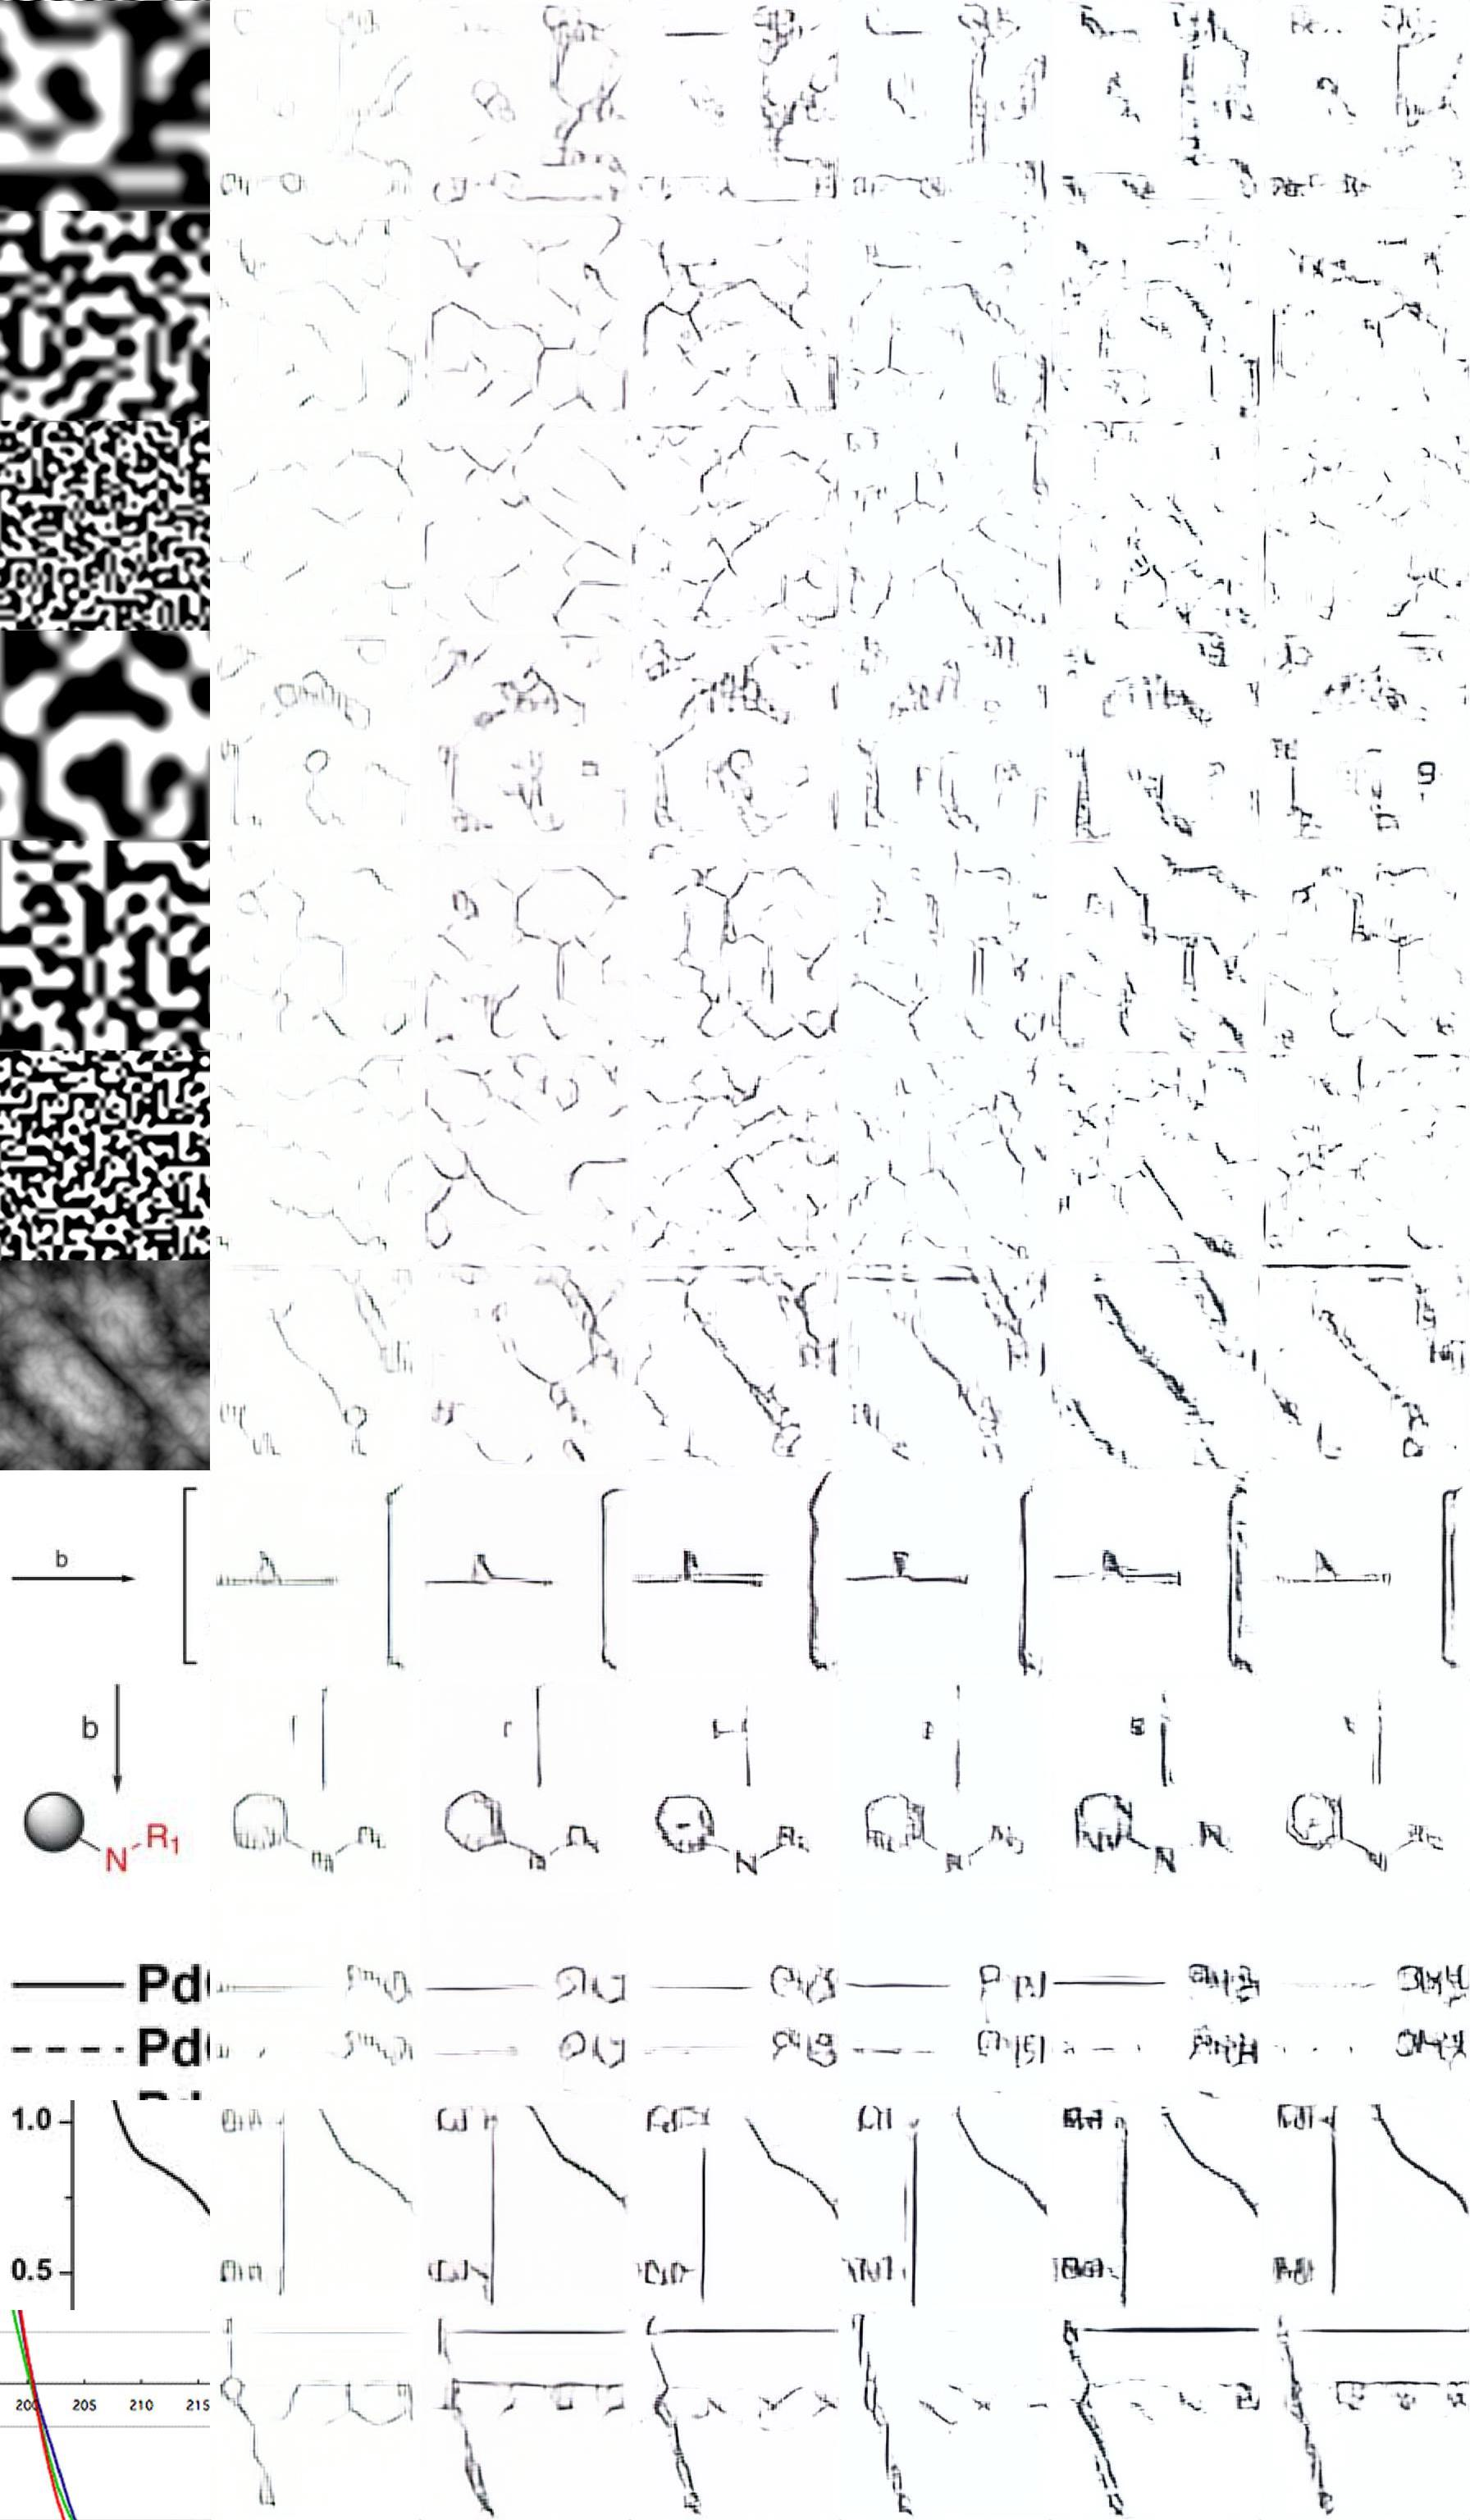
\includegraphics[scale=0.2]{imagenes/image_generation/256/256_2.jpg}}  
\end{figure}


\begin{figure}[H]
\centering
    \caption{Resultados de entrenar los modelos sobre el conjunto de datos con \textit{data augmentation} 1. La primera columna representa la imagen de entrada, el resto los diferentes modelos entrenados desde 70 hasta 170 épocas, tomadas de 20 en 20.} 
    \fbox{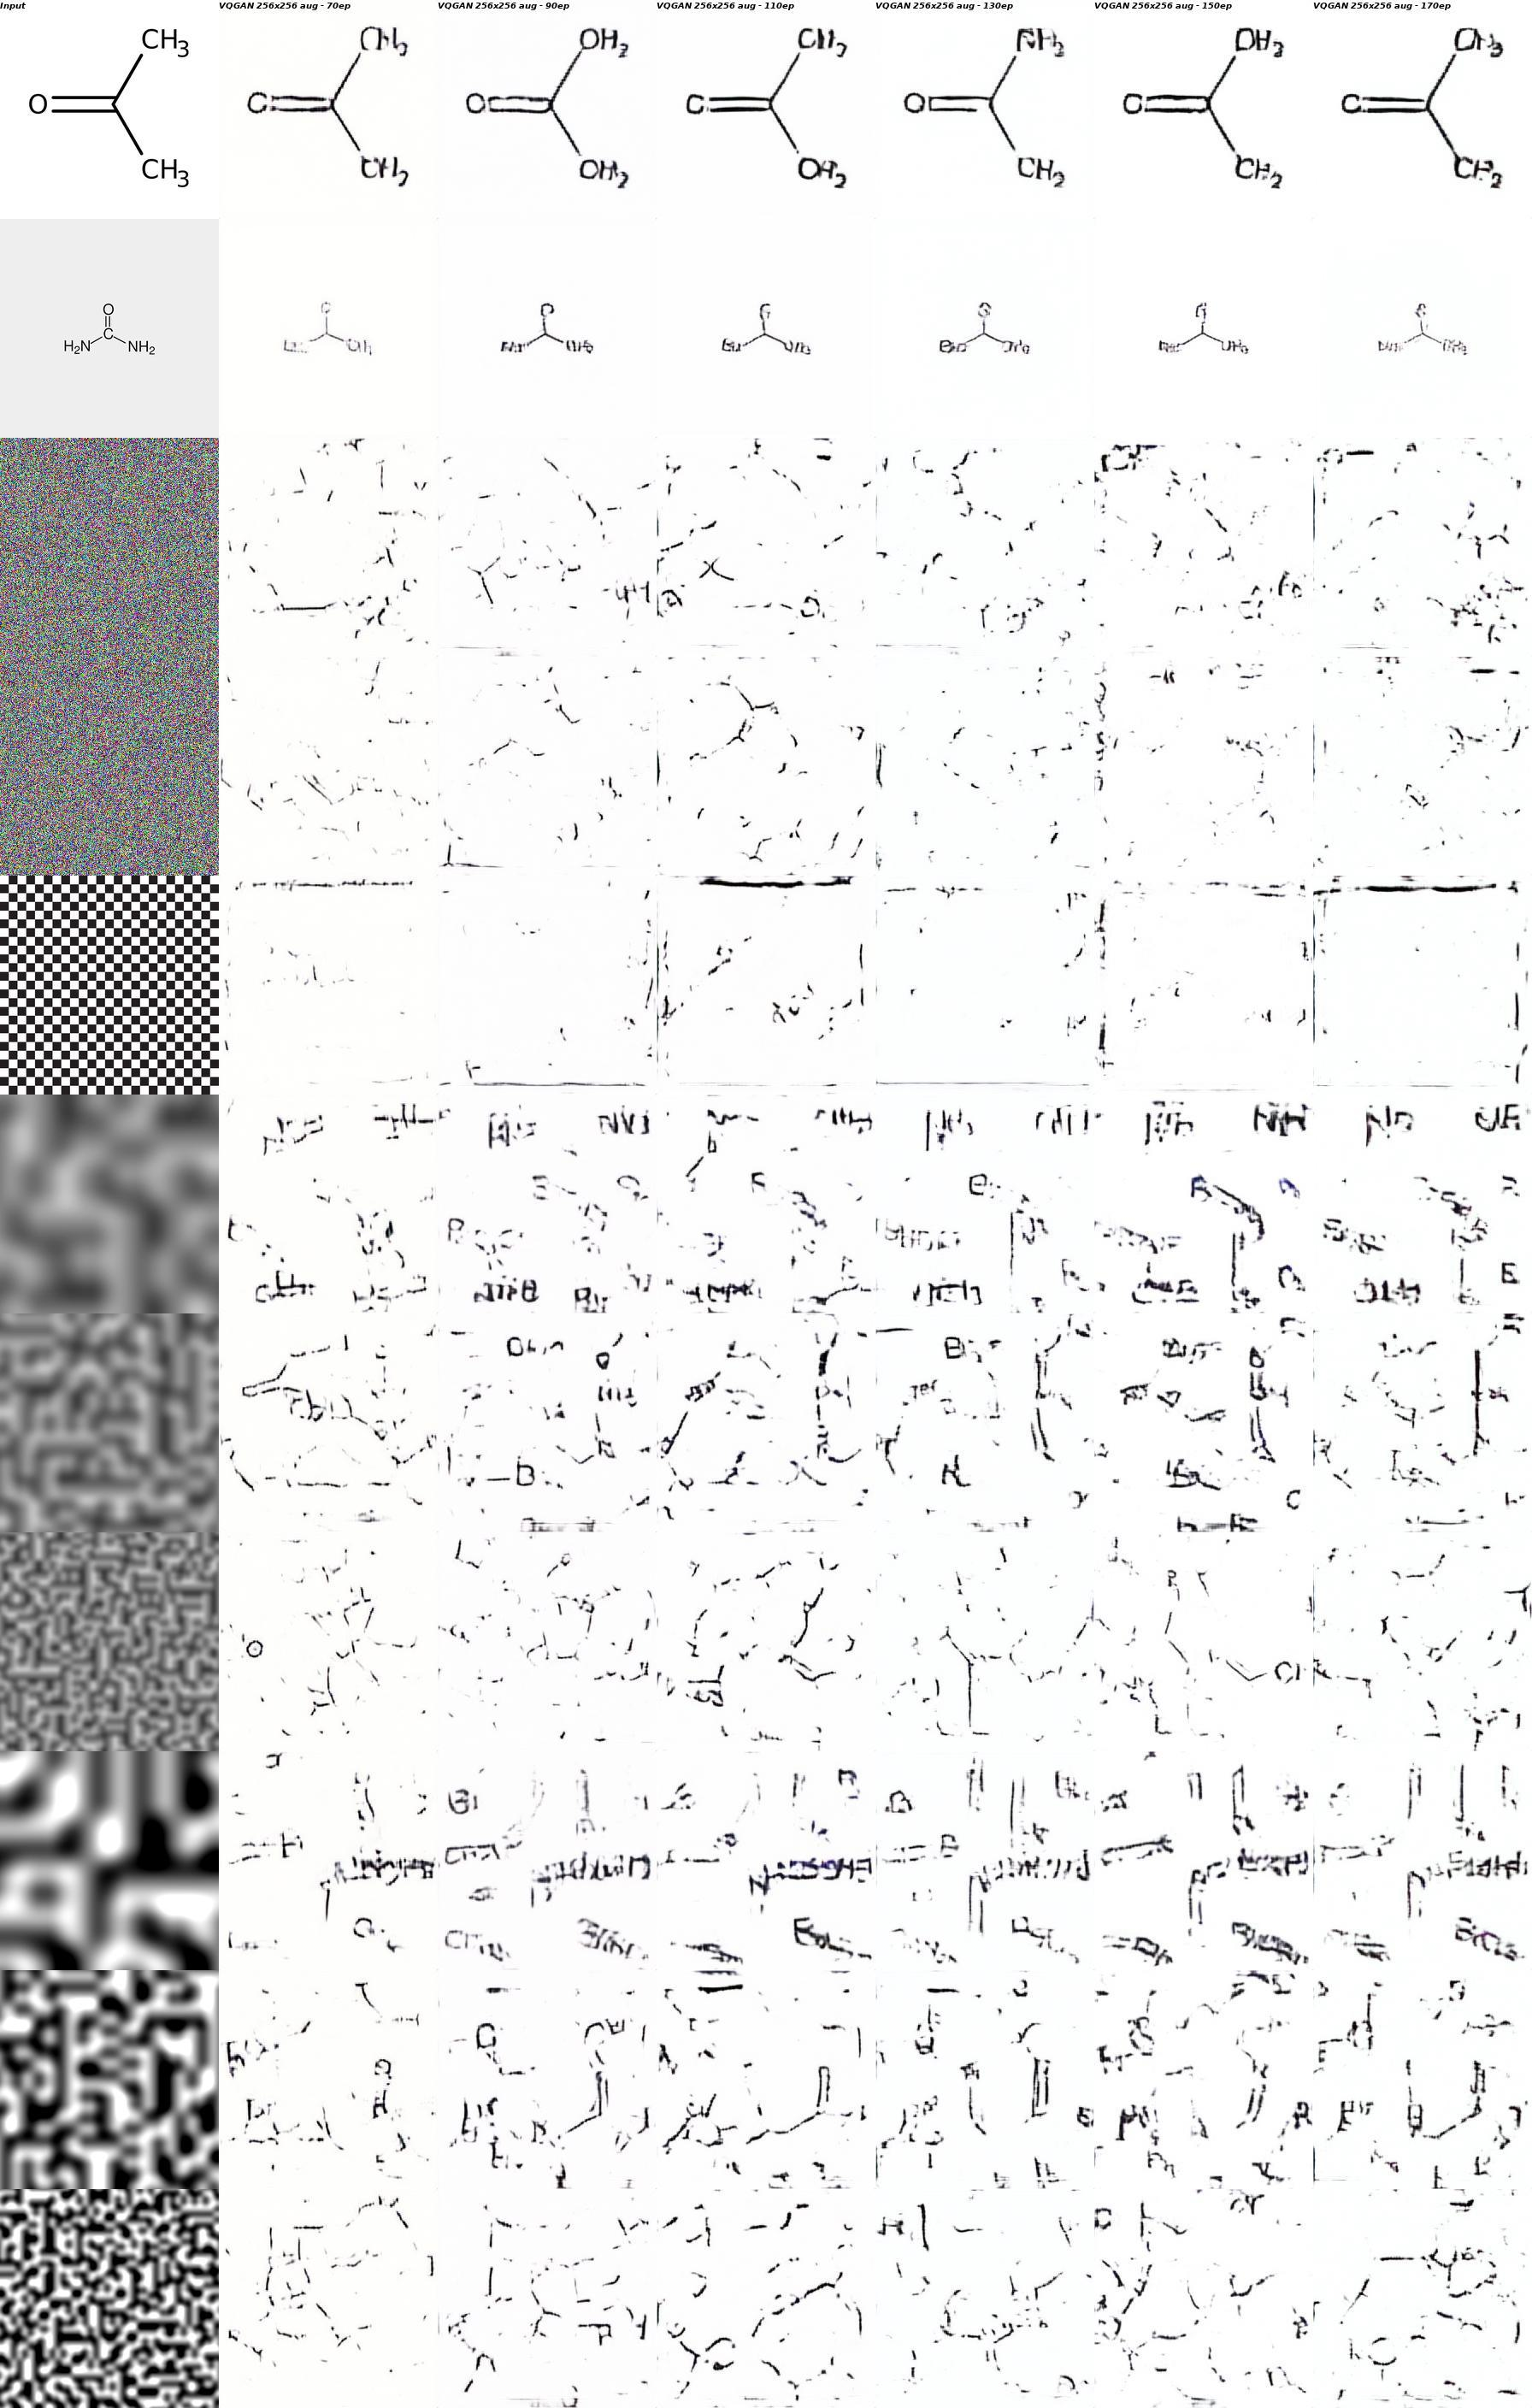
\includegraphics[scale=0.2]{imagenes/image_generation/256/aug_1.jpg}}  
\end{figure}

\begin{figure}[H]
\centering
    \fbox{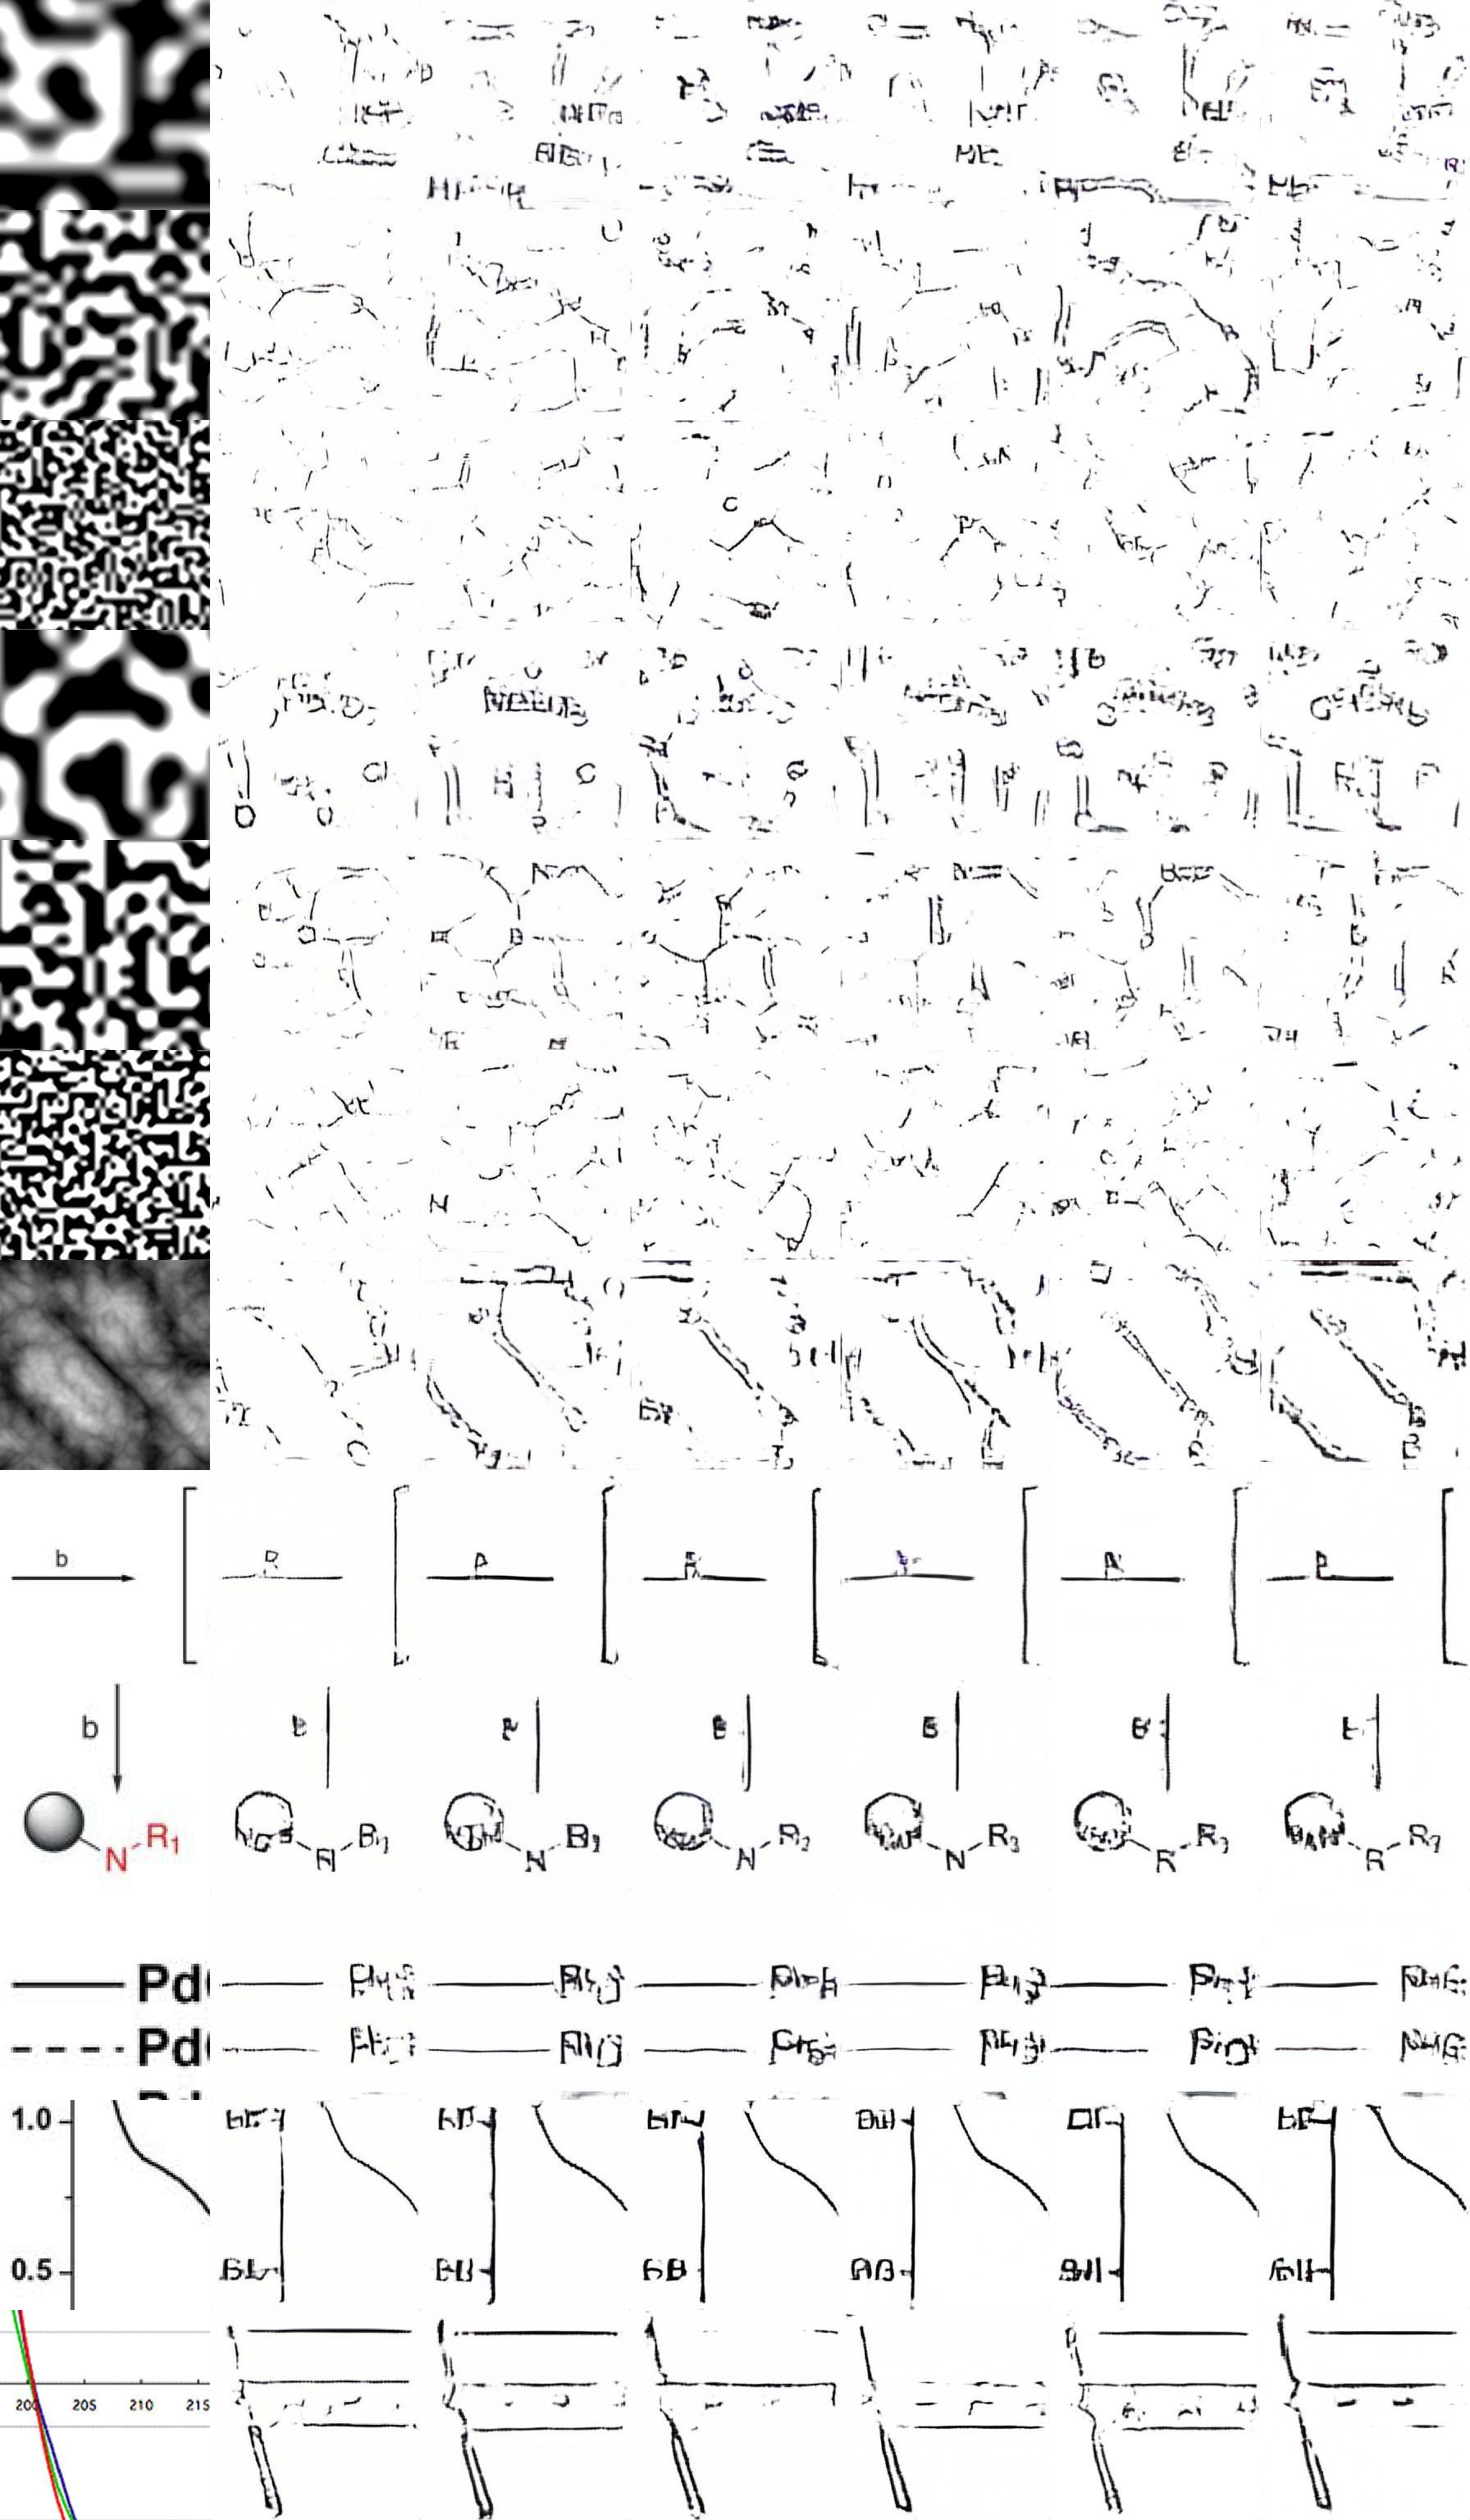
\includegraphics[scale=0.2]{imagenes/image_generation/256/aug_2.jpg}}  
\end{figure}


\begin{figure}[H]
\centering
    \caption{Resultados de entrenar los modelos sobre el conjunto de datos con \textit{data augmentation} 2. La primera columna representa la imagen de entrada, el resto los diferentes modelos entrenados desde 70 hasta 170 épocas, tomadas de 20 en 20.} 
    \fbox{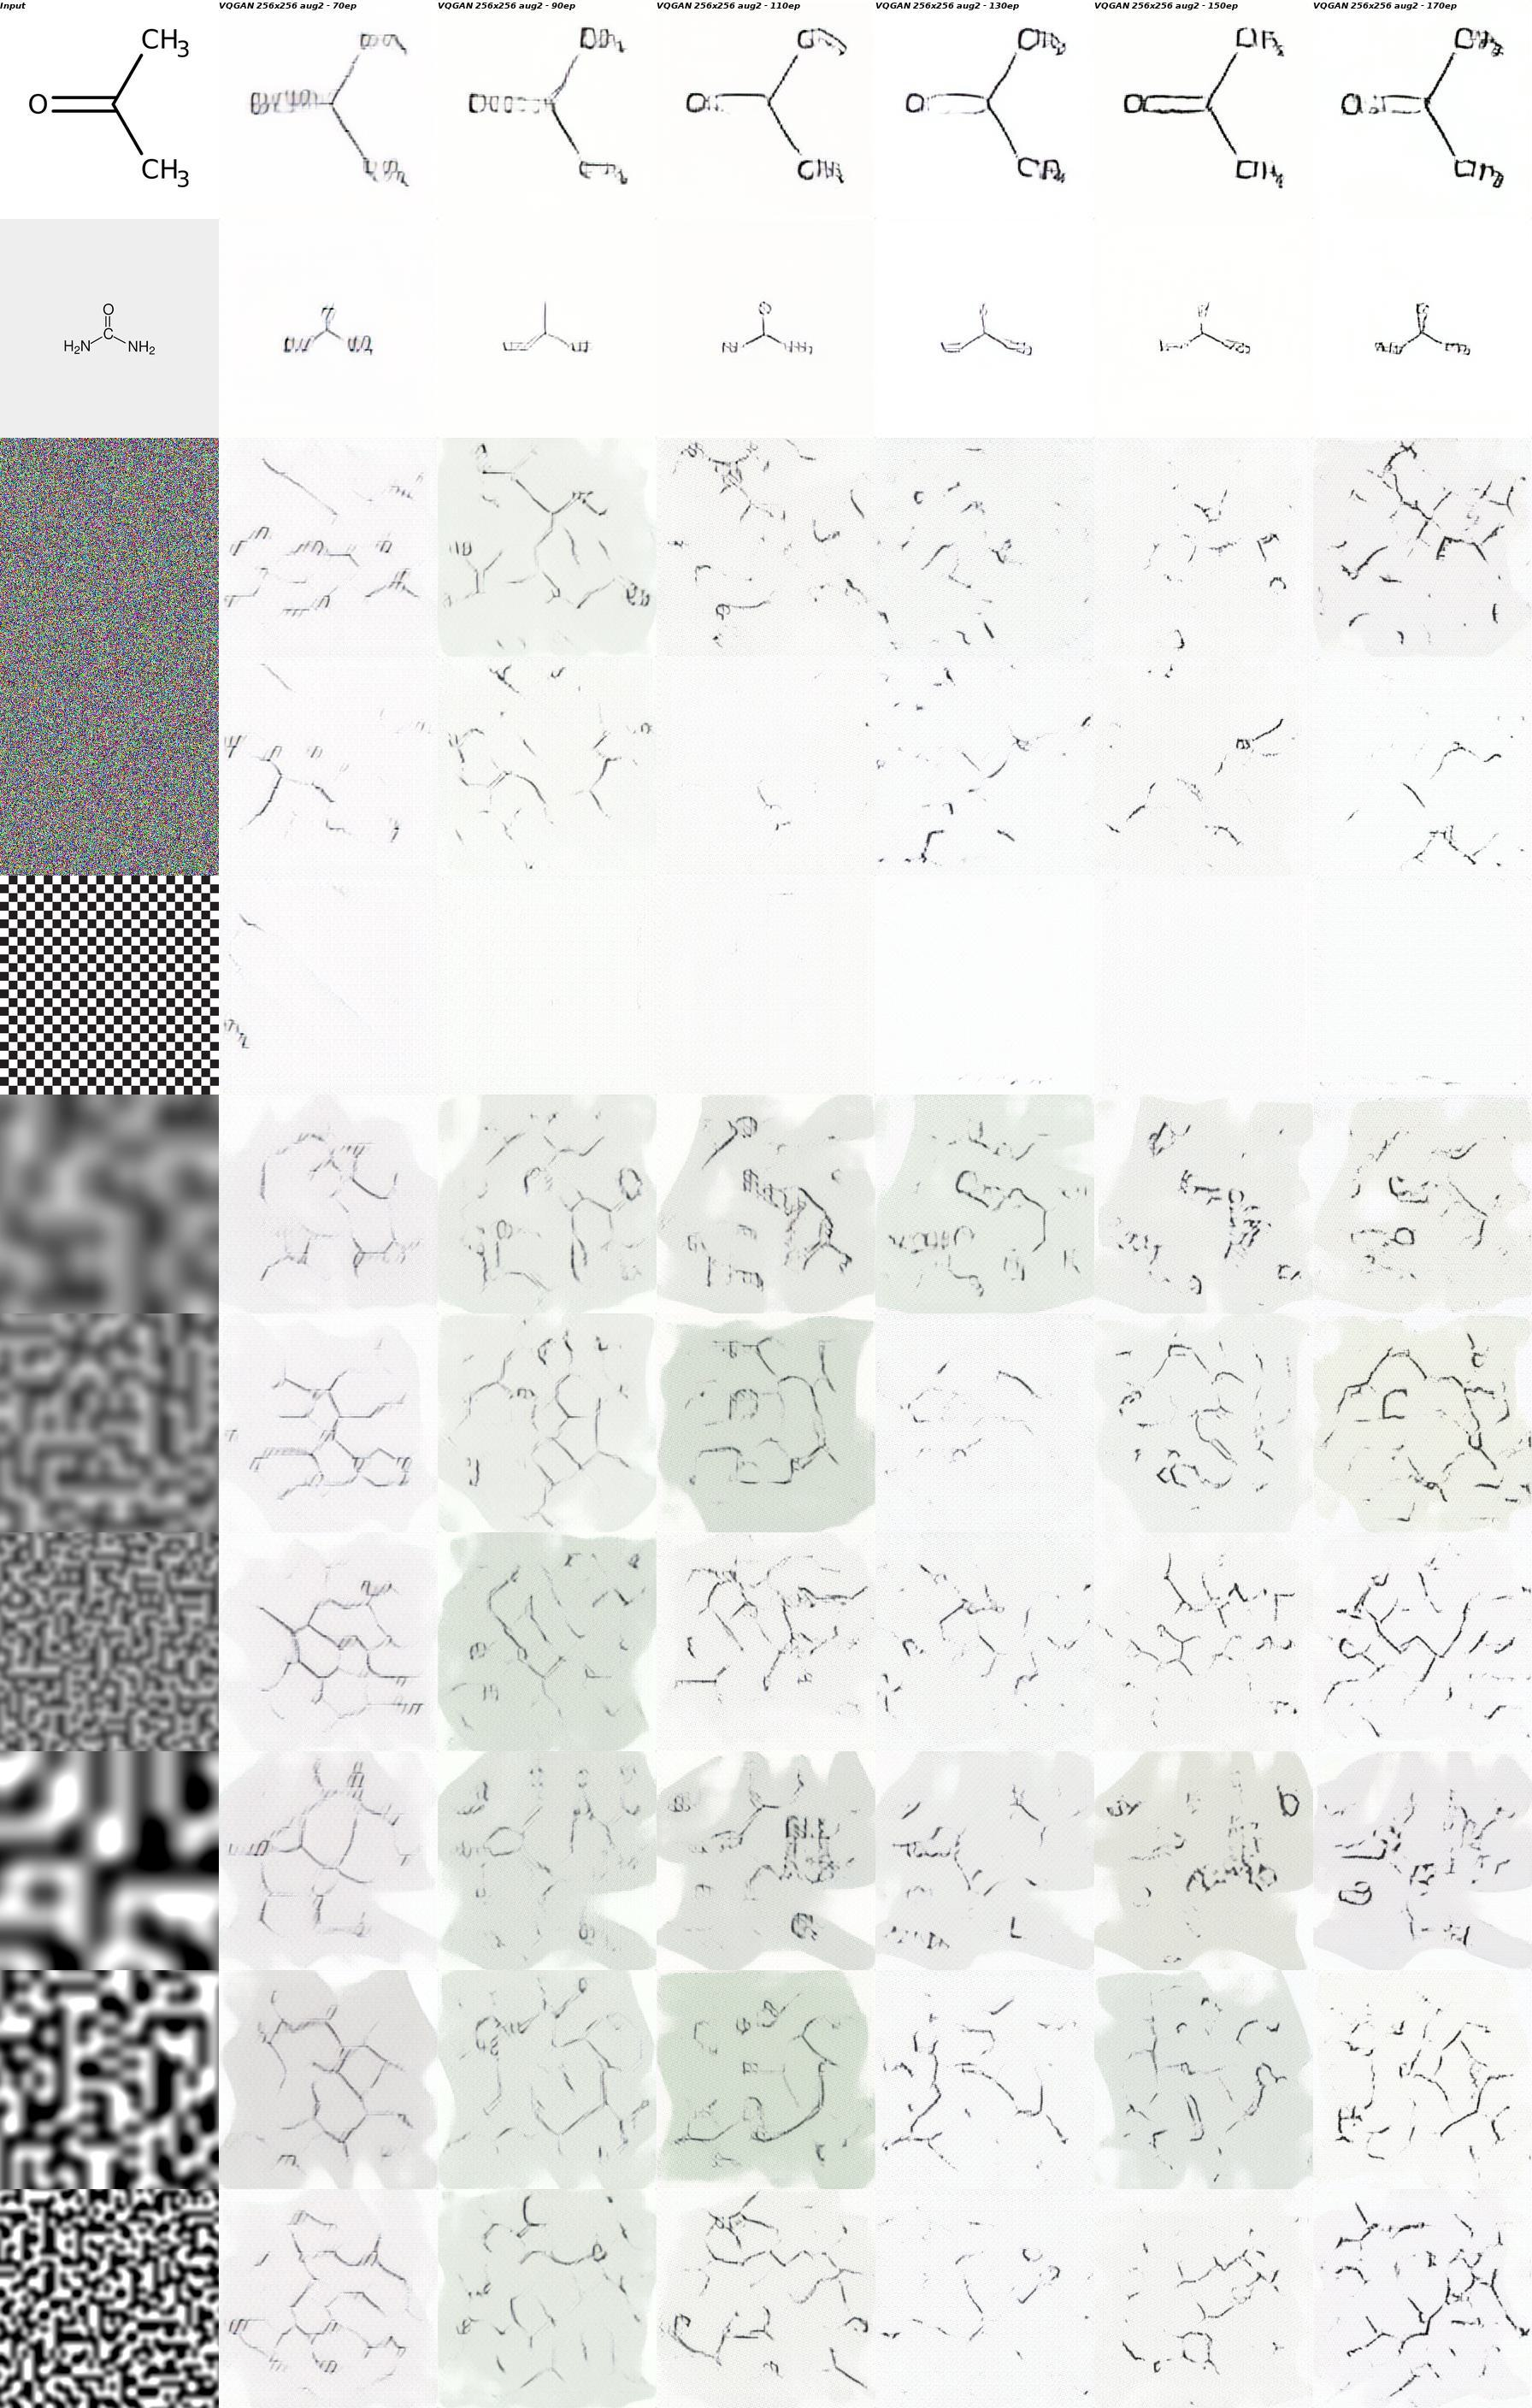
\includegraphics[scale=0.2]{imagenes/image_generation/256/aug2_1.jpg}}  
\end{figure}

\begin{figure}[H]
\centering
    \fbox{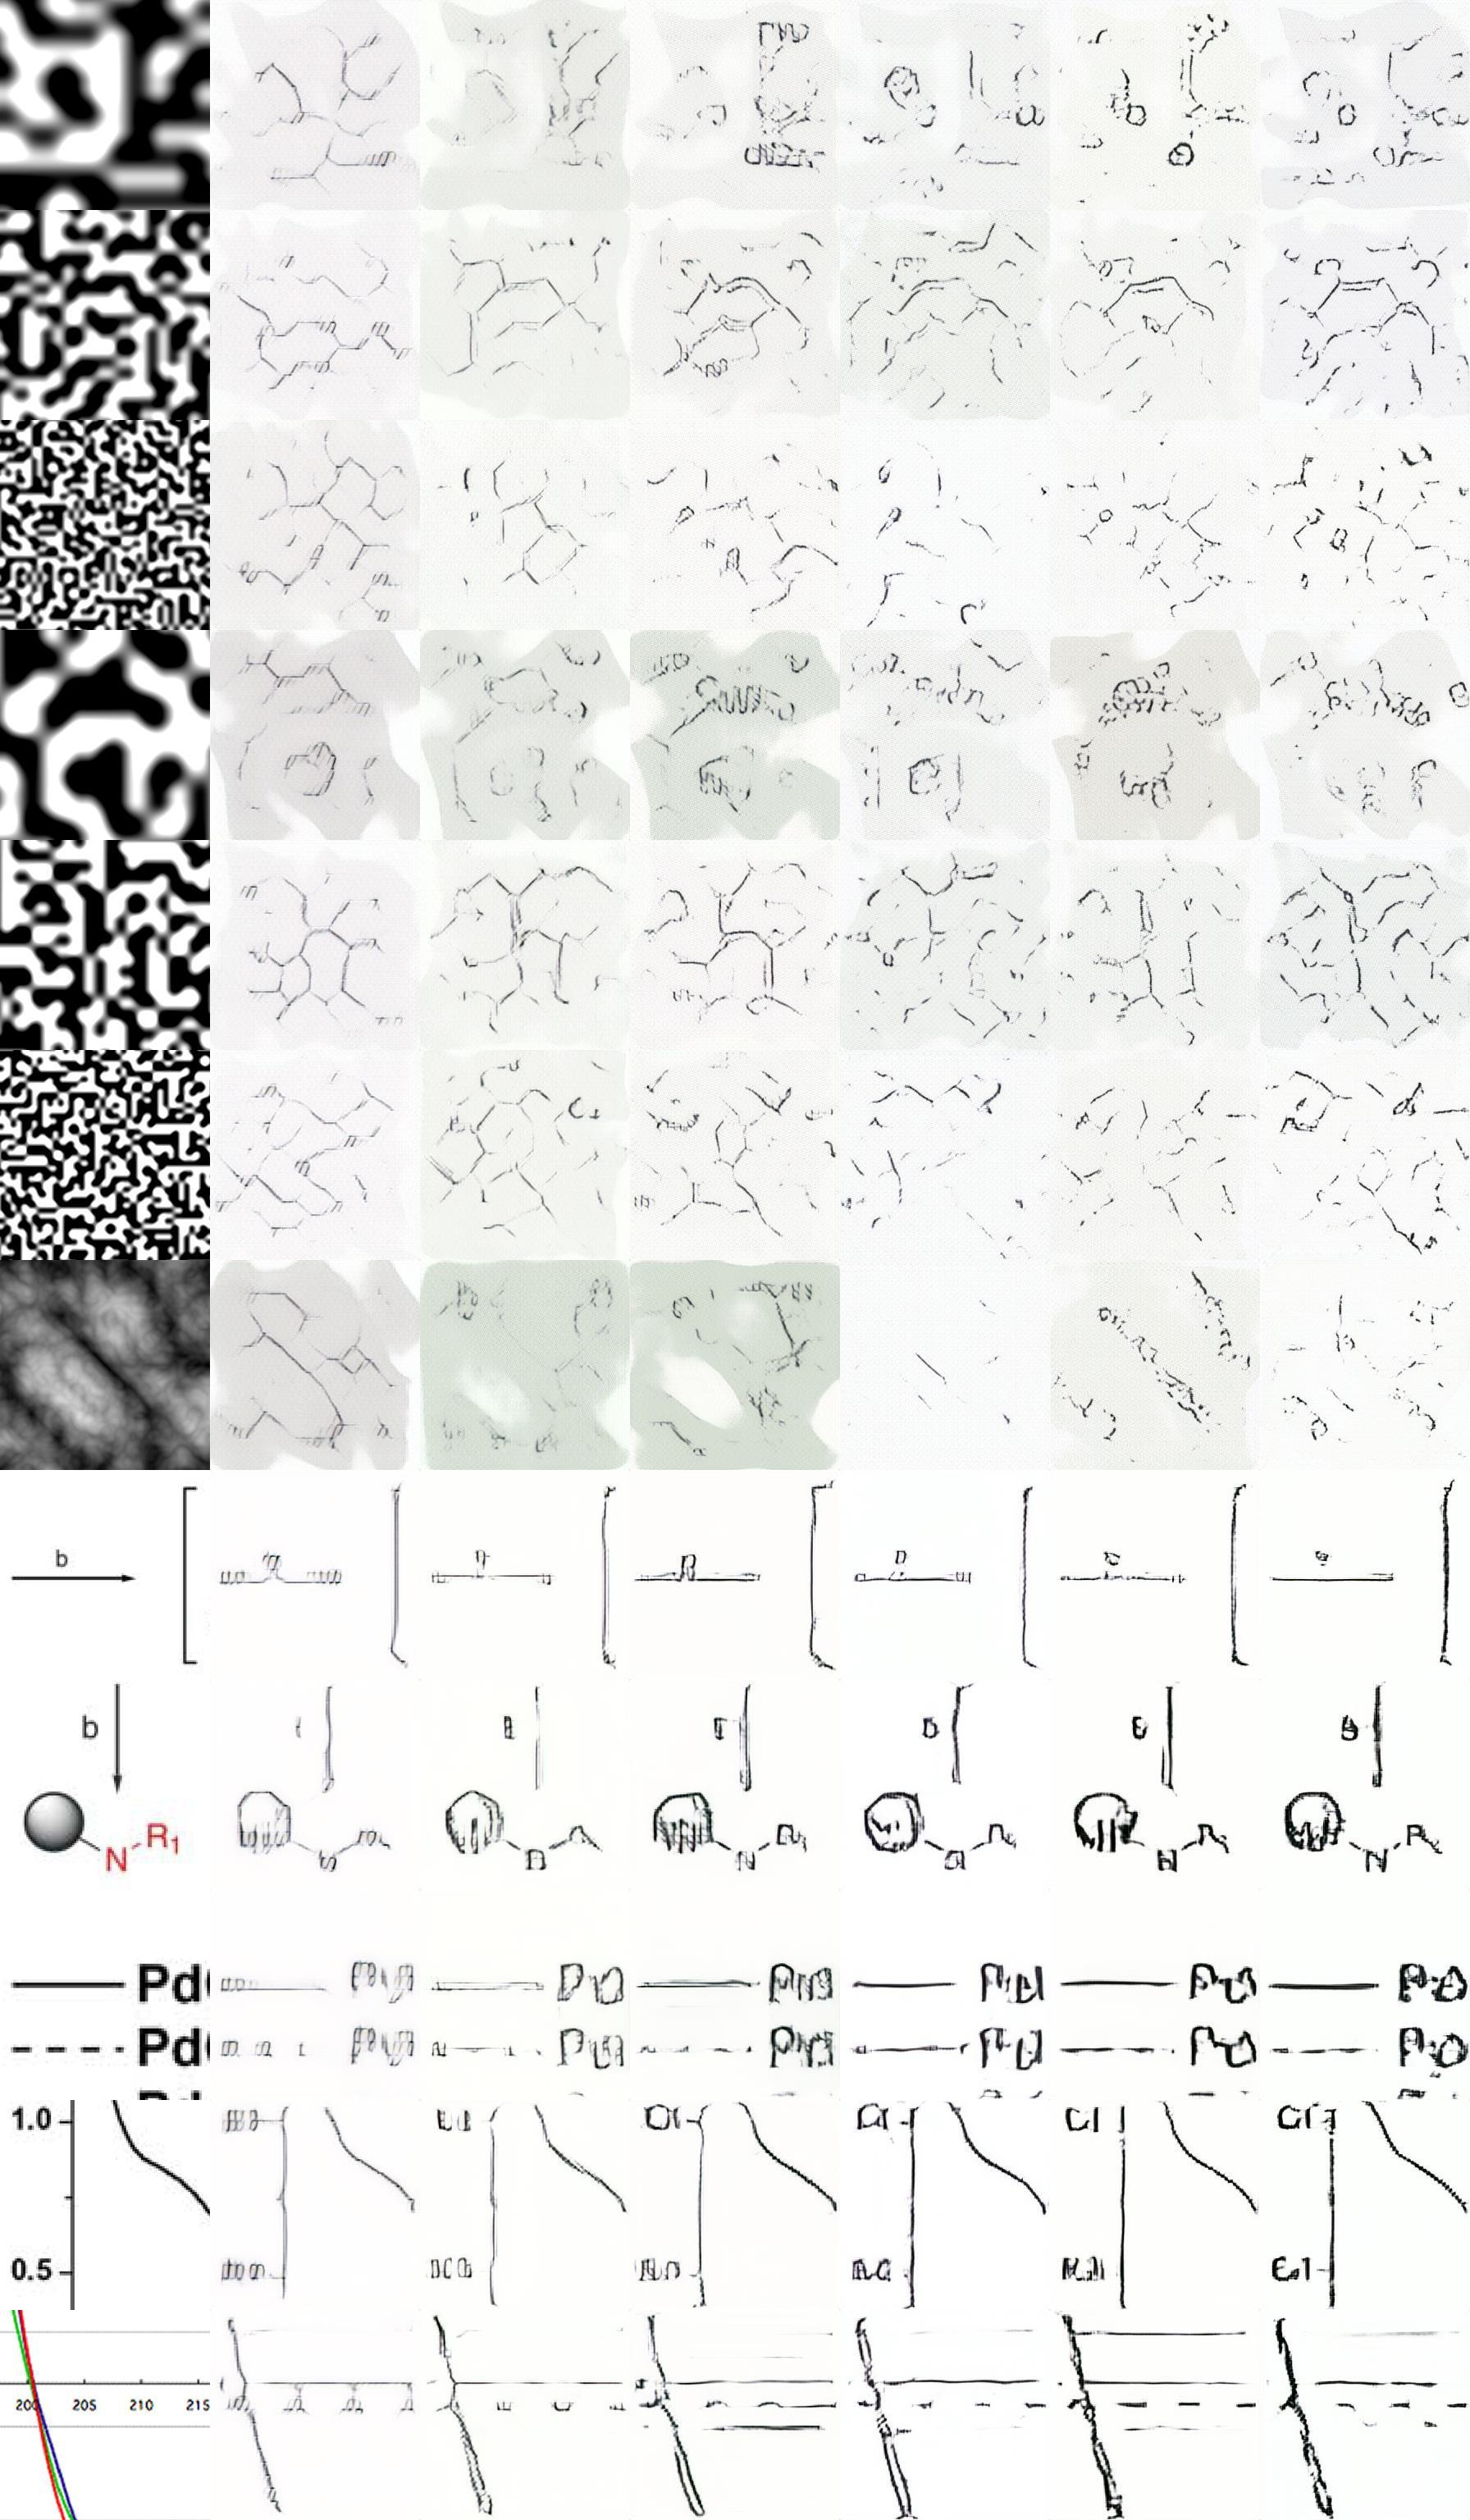
\includegraphics[scale=0.2]{imagenes/image_generation/256/aug2_2.jpg}}  

\end{figure}


\begin{figure}[H]
\centering
    \caption{Resultados de entrenar los modelos sobre el conjunto de datos con \textit{data augmentation} 3. La primera columna representa la imagen de entrada, el resto los diferentes modelos entrenados desde 70 hasta 170 épocas, tomadas de 20 en 20.}
    \fbox{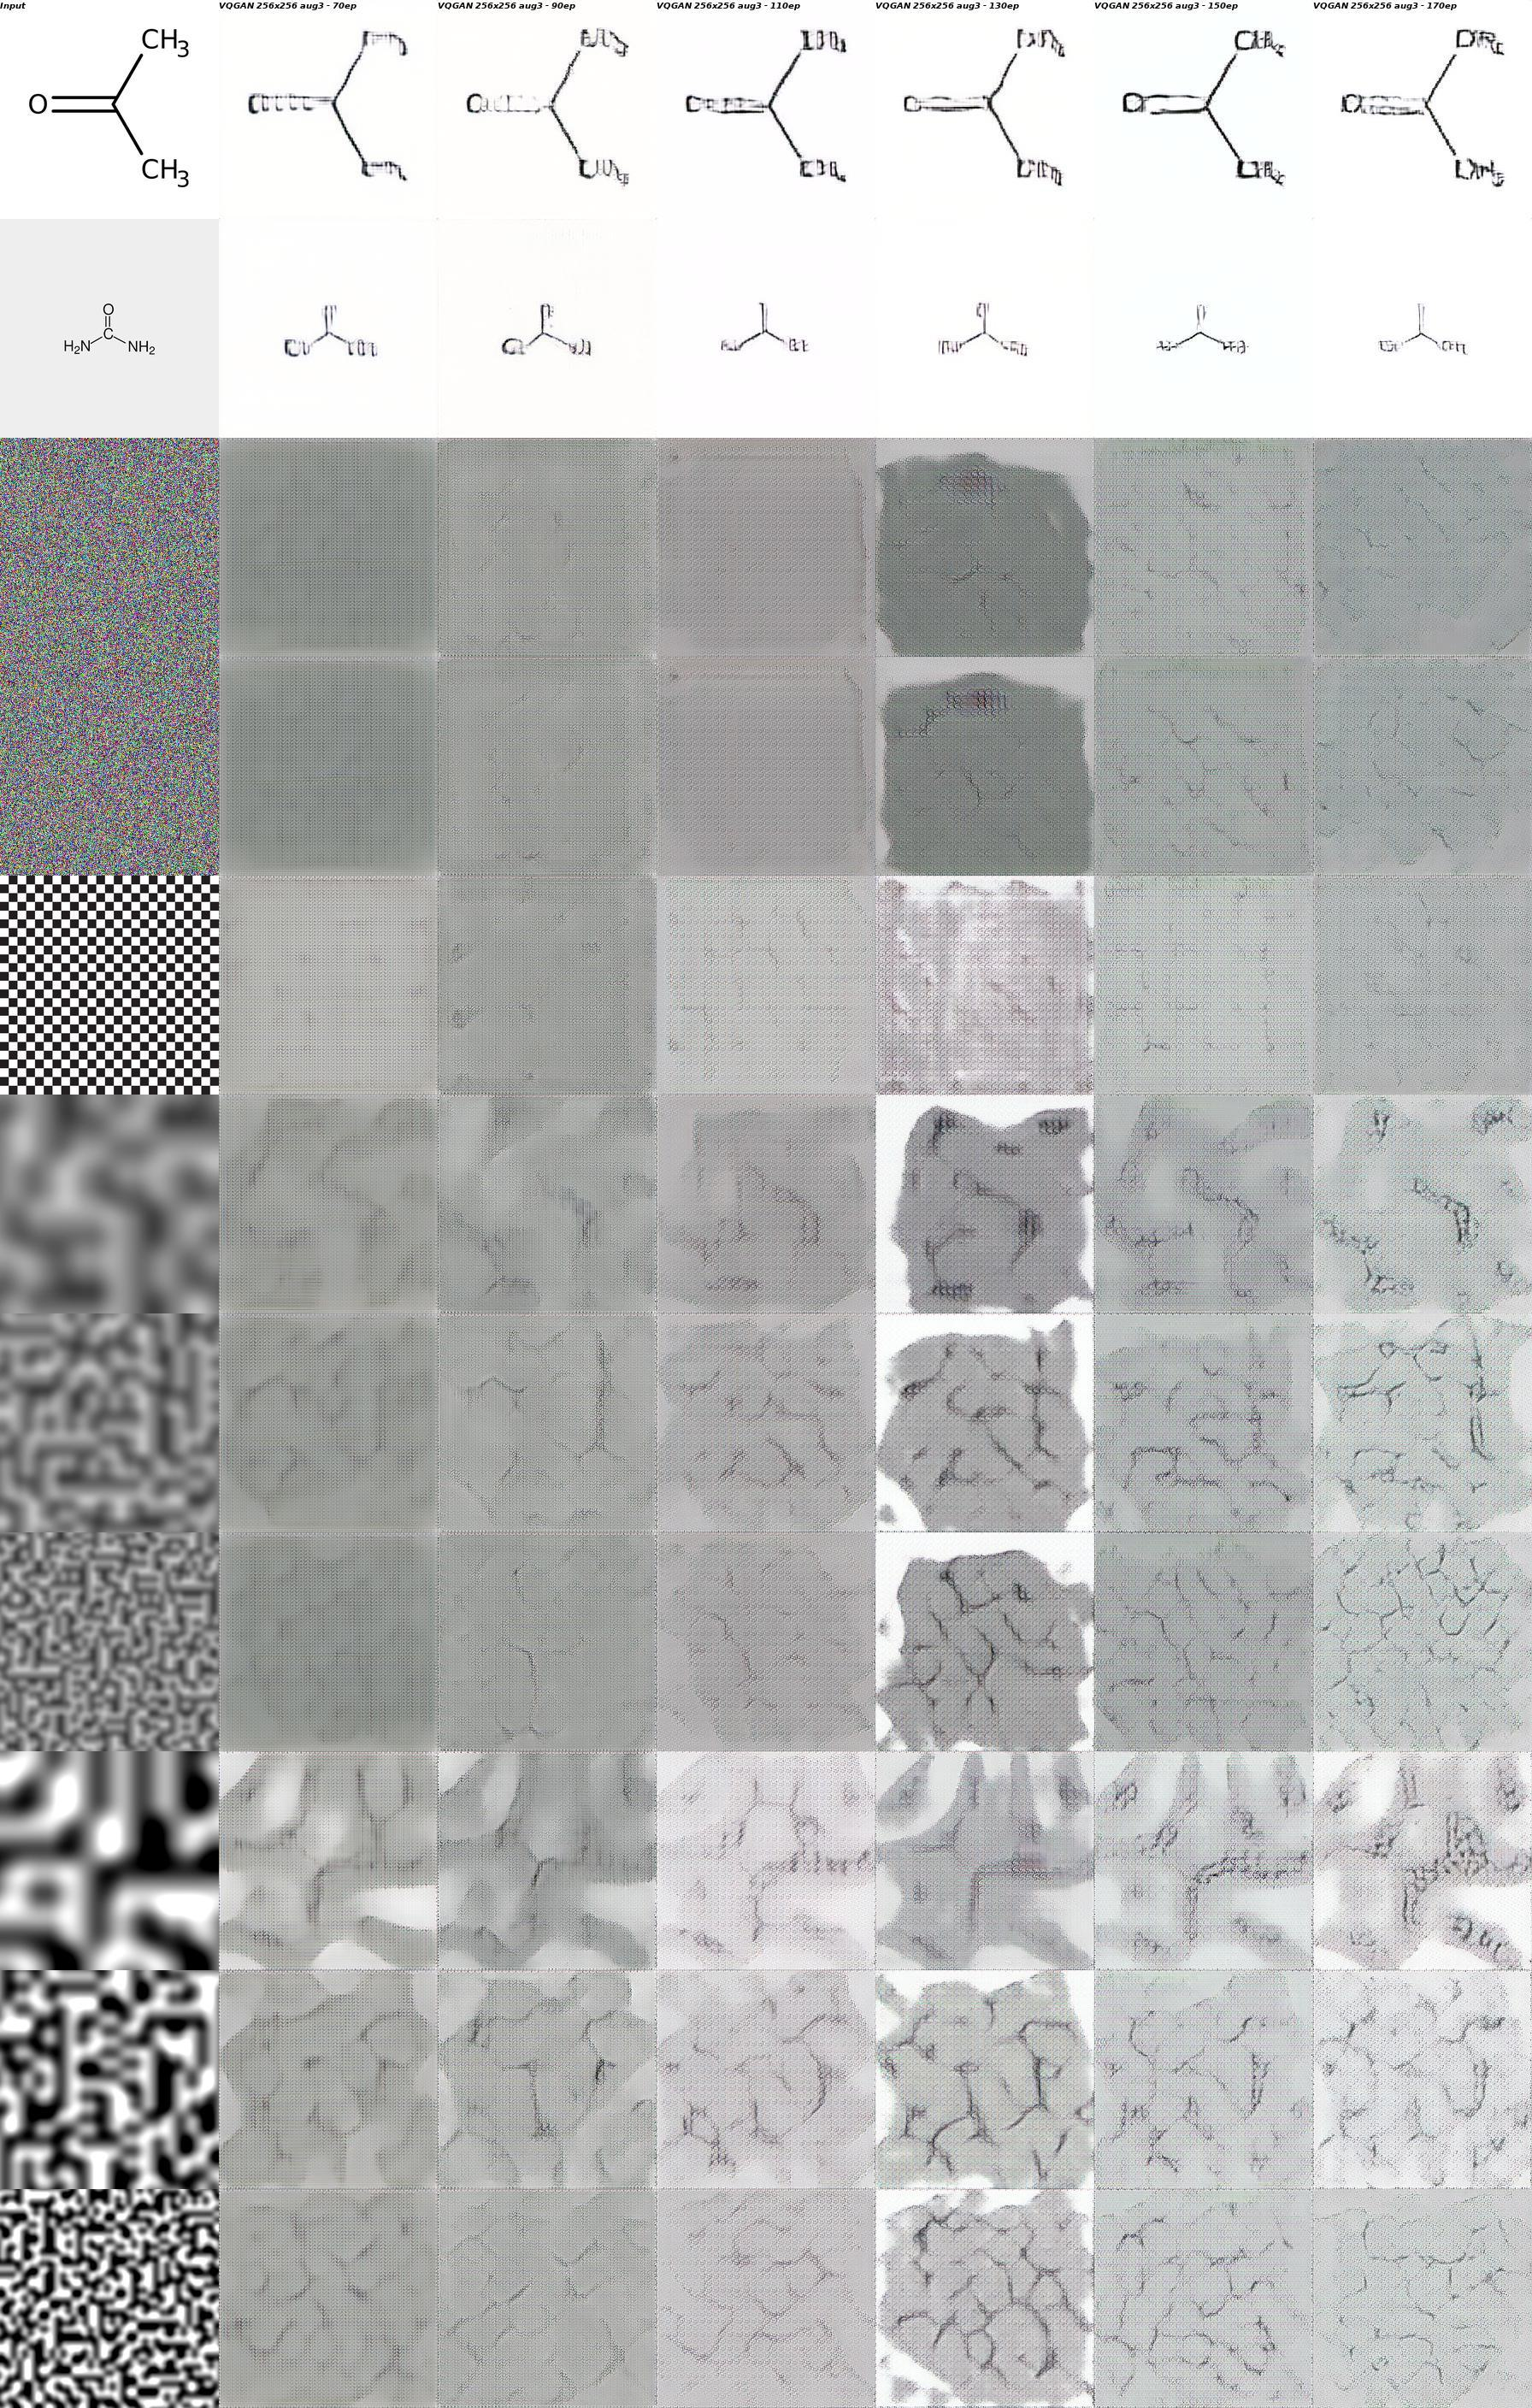
\includegraphics[scale=0.2]{imagenes/image_generation/256/aug3_1.jpg}}  
\end{figure}

\begin{figure}[H]
\centering
    \fbox{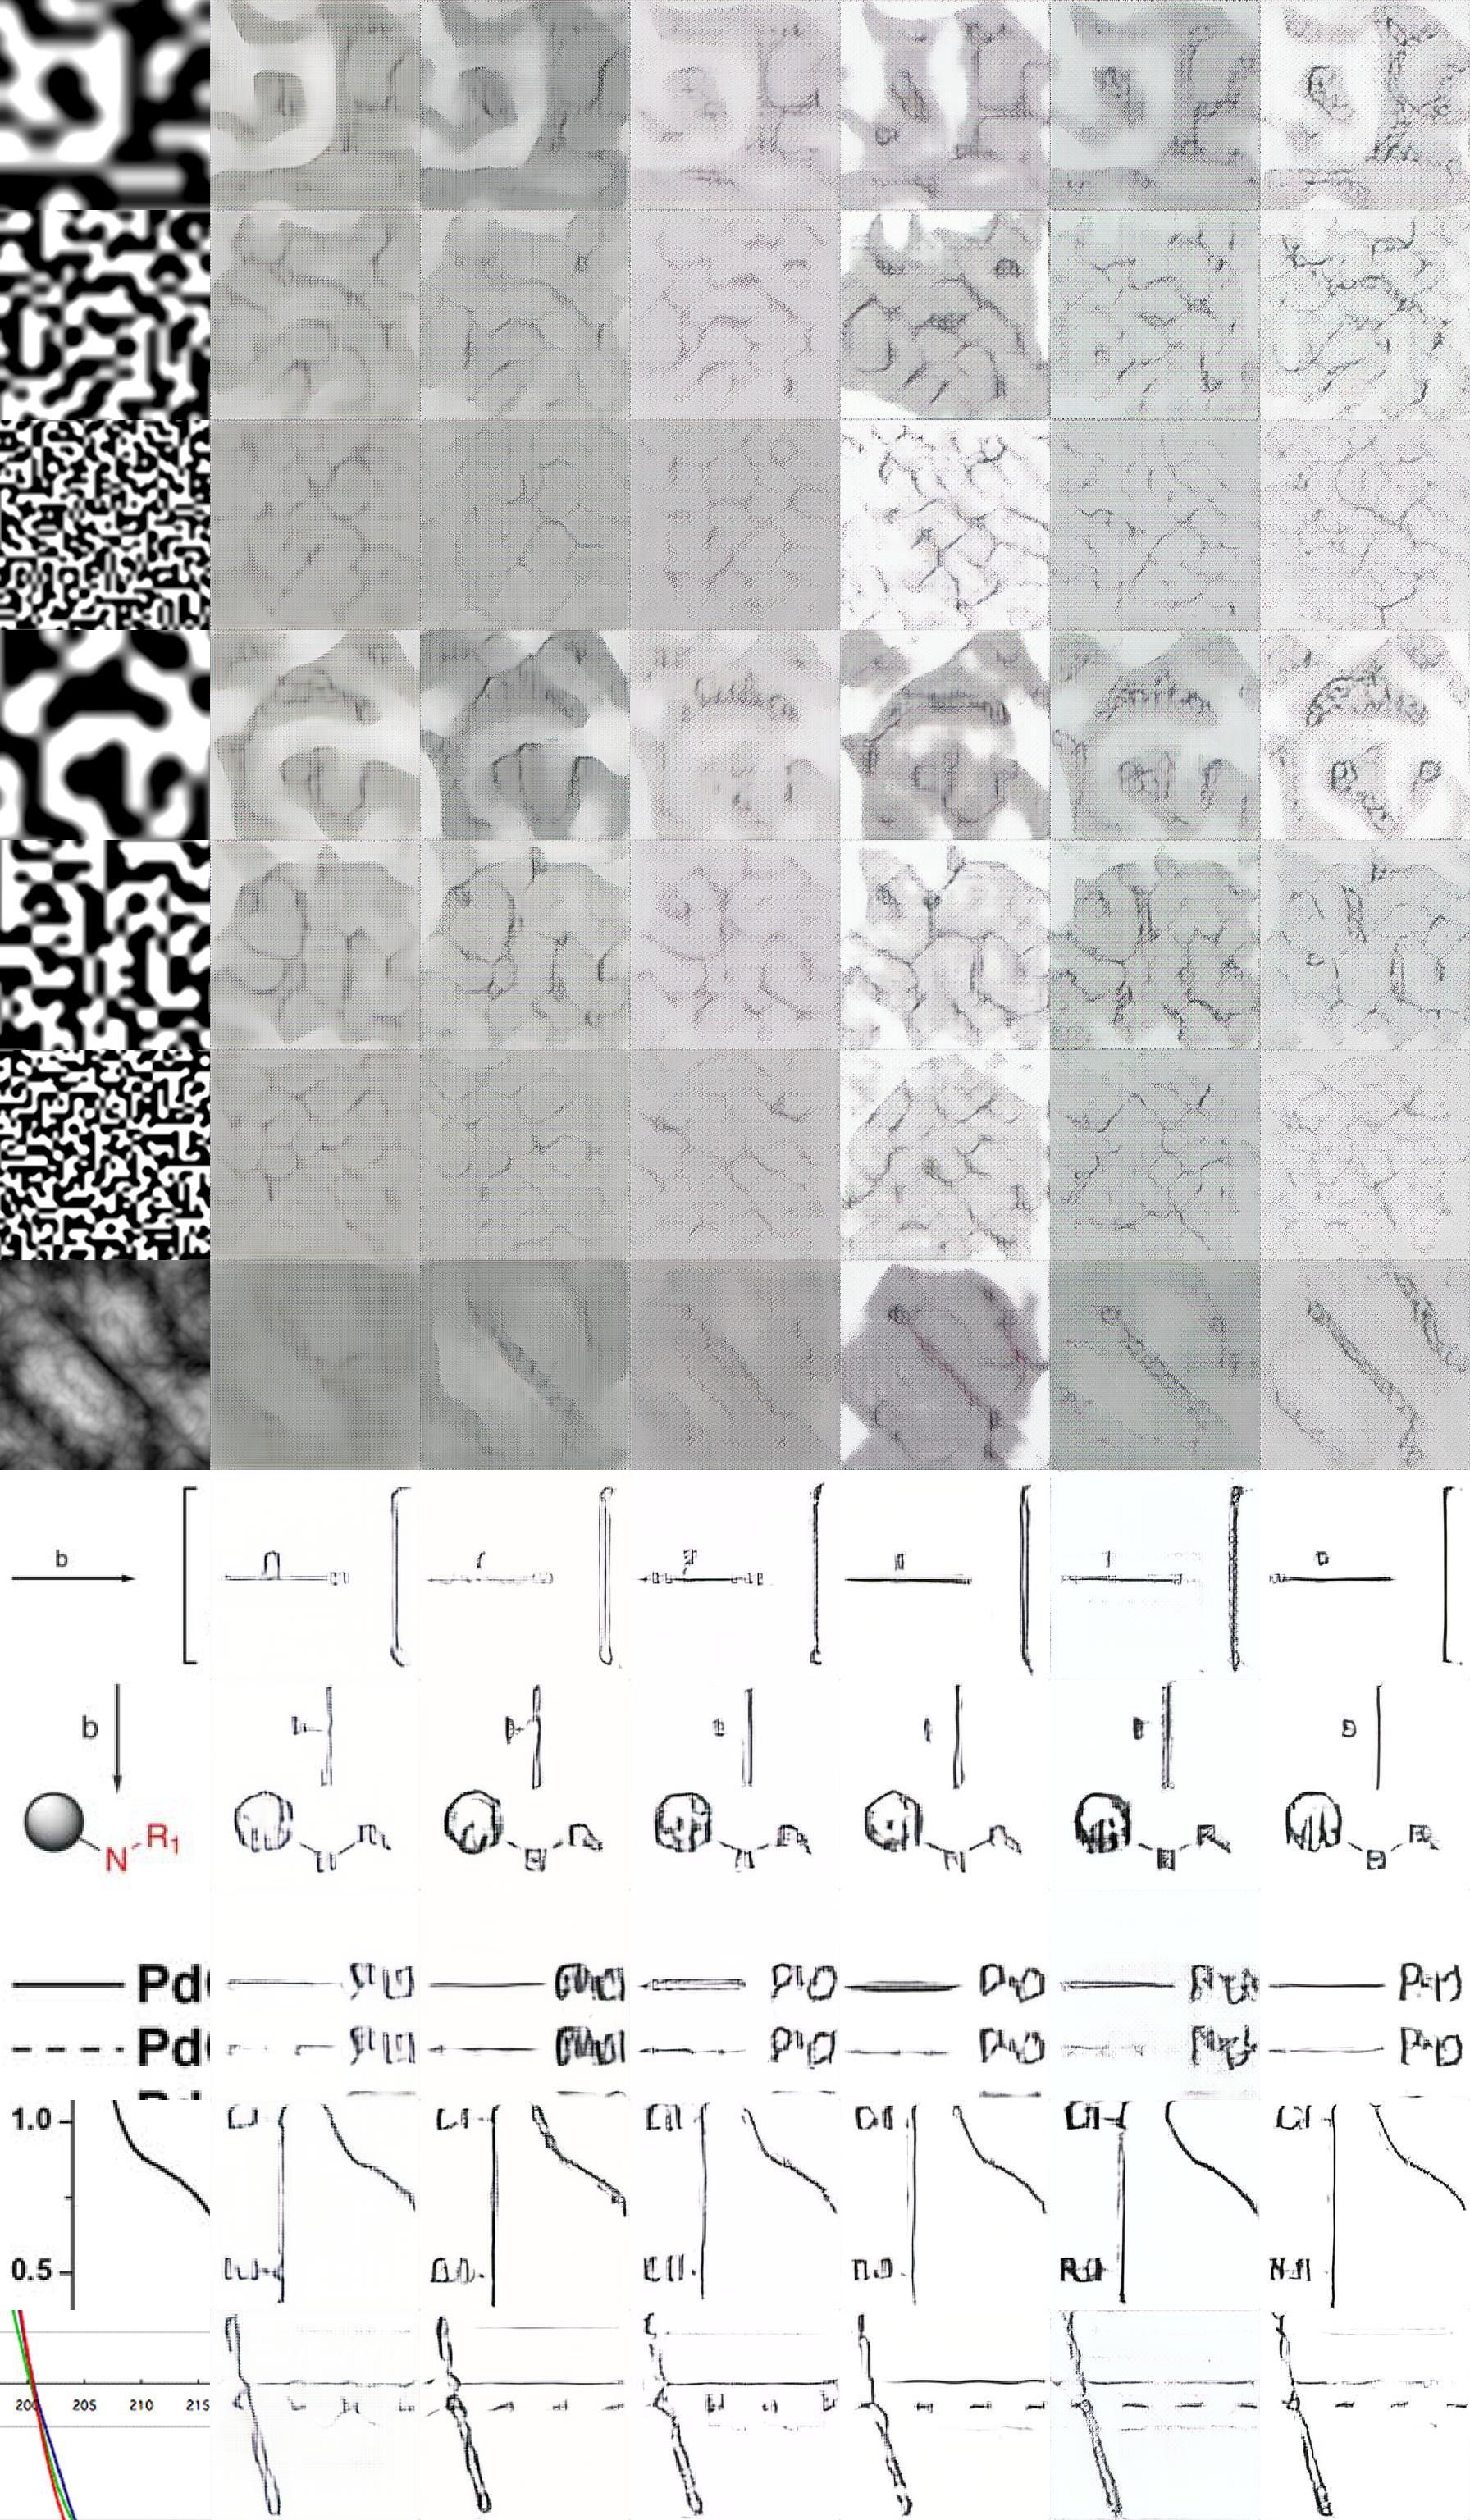
\includegraphics[scale=0.2]{imagenes/image_generation/256/aug3_2.jpg}}  
\end{figure}

Los resultados fueron mostrados a los científicos israelíes, y decidieron que los obtenidos con \textit{data augmentation} 2 se acercaban a lo que querían.

¿Qué tipo de datos de entrada se ha utilizado para generar las imágenes sintéticas? En un primer momento probamos a utilizar imágenes de moléculas reales y de objetos que sin ser moléculas, lo parecen. En el primer caso, la salida es similar a la entrada, con la diferencia de que la imagen sintética pierde información: detalles como letras o números se alteran. En el segundo caso ocurre algo similar, con la particularidad de que objetos circulares son transformados en formas que parecen hexágonos propios de las moléculas. Además, incluso se añaden átomos.

\begin{figure}[H]
\centering
    \fbox{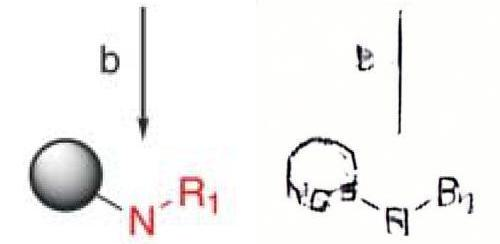
\includegraphics[scale=0.3]{imagenes/image_generation/256/circle_to_hex.jpg}}
    \caption{El modelo tiene la capacidad de modificar la imagen para que se parezca a una molécula.}
\end{figure}

Pero nuestro objetivo es poder generar tantas imágenes como queramos, así que deberíamos poder partir de una imagen de entrada generada aleatoriamente. En un primer momento se utilizó ruido uniforme, pero no funcionó bien en ningún caso. Este tipo de ruido no sigue ninguna estructura, y nuestro modelo necesita algún tipo de entrada que tenga cierta continuidad. Por ello probamos con una cuadrícula de ajedrez: ocurre lo mismo, ya que aunque existe un patrón que se repite, los elementos de este no están conectados entre sí.

\subsection{Ruido Perlín}
Se trata de un ruido inventado por Ken Perlin en 1982 que revolucionó el ámbito de la Informática Gráfica. En esta rama de las Ciencias de la Computación, la creación de texturas que imitan materiales de la naturaleza como la madera o el mármol es una tarea importante. Generar estas texturas de una forma manual o mediante un escáner no es una opción escalable.

Este ruido permite simular fenómenos que requieran aleatoriedad a la vez que continuidad. Para ello, genera una serie de gradientes en un grid (en nuestro caso 2D). A continuación, interpola el valor de esos gradientes mediante interpolación polinómica de Hermite. La ventaja de este ruido frente a otros que también se generan mediante interpolación es su eficiencia, para calcular la interpolación en un punto solo intervienen los $2^n$ gradientes más cercanos, donde $n$ es el número de dimensiones.

\begin{figure}[H]
\centering
    \fbox{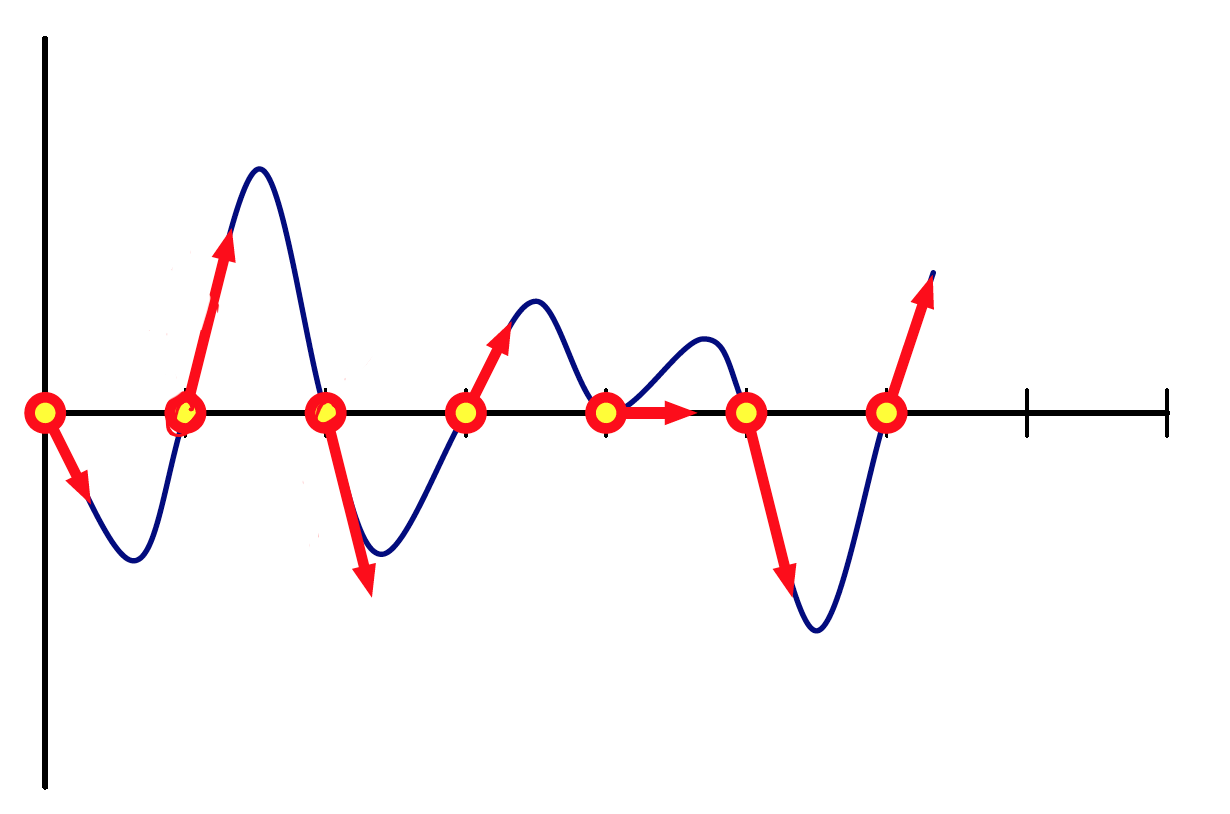
\includegraphics[scale=0.3]{imagenes/image_generation/perlin_interpolation.png}}
    \caption{Interpolación de gradientes en el Ruido Perlín 1D.}
\end{figure}

El Ruido Perlín se puede modificar cambiando la amplitud y frecuencia de este. A mayor amplitud, los cambios entre zonas del ruido serán más bruscos, a menor amplitud el ruido será más homogéneo y suave. La frecuencia cambia la granularidad del ruido, a mayor frecuencia encontramos un grano más fino. 

\begin{figure}[H]
\centering
    \begin{subfigure}{.26\textwidth}
        \centering
        
\includegraphics[width=1\linewidth]{imagenes/image_generation/perlin_python_3_1.jpg}
        \caption{Amp:3 Frec:1}
    \end{subfigure}%
    \begin{subfigure}{.26\textwidth}
        \centering
        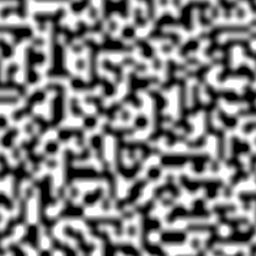
\includegraphics[width=1\linewidth]{imagenes/image_generation/perlin_python_3_4.jpg}
        \caption{Amp:3 Frec:4}
    \end{subfigure}%

    \bigskip

    \begin{subfigure}{.26\textwidth}
        \centering
        
\includegraphics[width=1\linewidth]{imagenes/image_generation/perlin_python_7_1.jpg}
        \caption{Amp:7 Frec:1}
    \end{subfigure}%
    \begin{subfigure}{.26\textwidth}
        \centering
        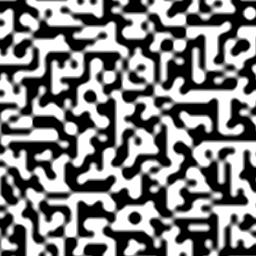
\includegraphics[width=1\linewidth]{imagenes/image_generation/perlin_python_7_4.jpg}
        \caption{Amp:7 Frec:4}
    \end{subfigure}

    \caption{Ejemplos de Ruido Perlín con distinta amplitud y frecuencia.}
\end{figure}

Como se observa, al contrario que con el ruido uniforme, este tipo de ruido es capaz de generar imágenes que parecen moléculas. Su continuidad permite que el modelo tenga una estructura en la que basarse para realizar la generación. 

Tras realizar estos experimentos, se los enseñamos a los científicos de Israel para conocer su opinión. Están conformes con la versión \textit{data augmentation} 2 entrenada durante 70 épocas en aquellos casos en los que se utiliza Ruido Perlín como entrada. De todas formas, como se obtienen buenos resultados entre 70 y 90 épocas, vamos a entrenar con \textit{data augmentation} 2 durante 70, 75, 80, 85 y 90 épocas y a comparar los resultados.

\begin{figure}[H]
\centering
    \caption{Resultados de entrenar con imágenes con \textit{data augmentation} 2, modelos entrenados desde las 70 hasta las 90 épocas tomadas de 5 en 5.}
    \fbox{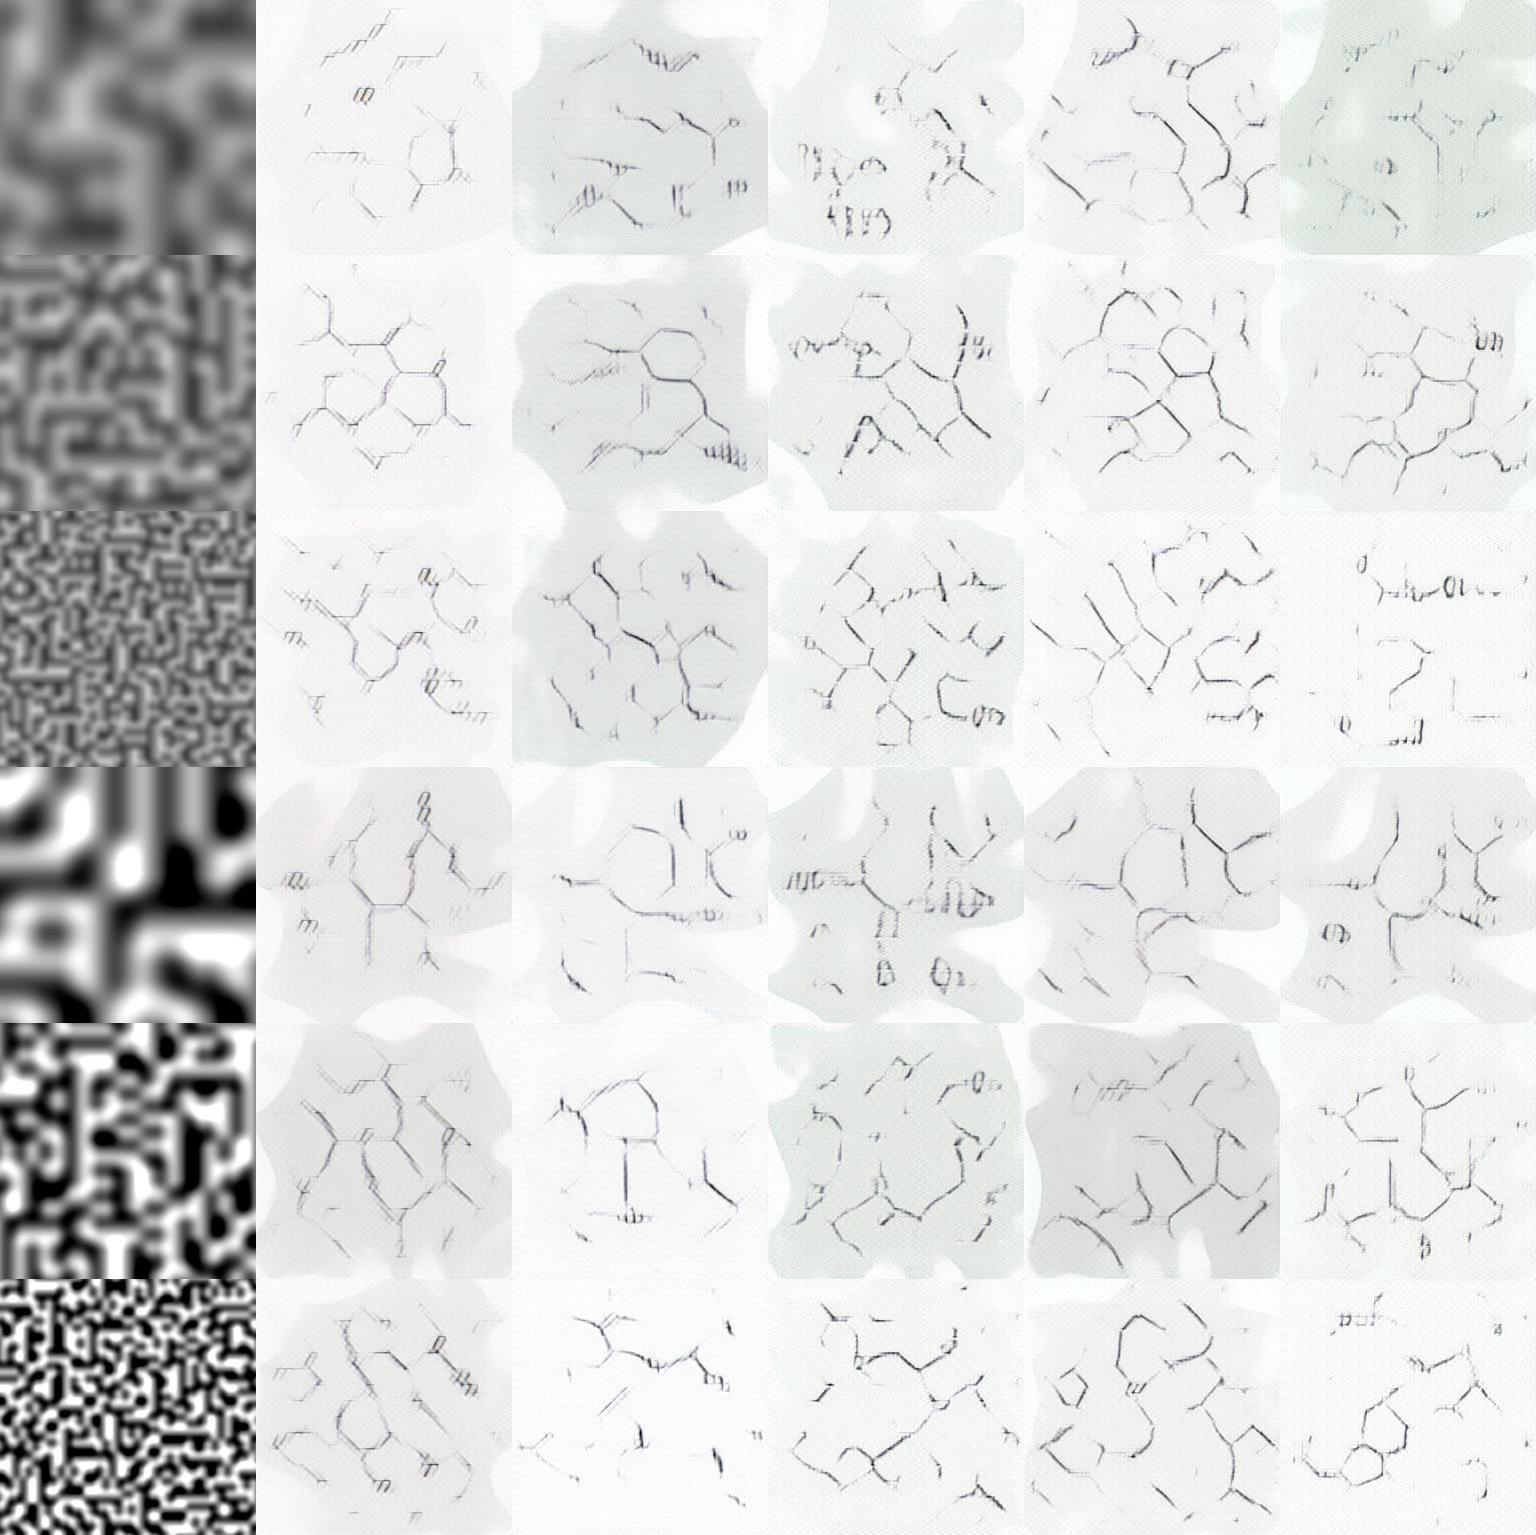
\includegraphics[scale=0.23]{imagenes/image_generation/256/aug2_extraepochs_1.jpg}}  
\end{figure}

\begin{figure}[H]
\centering
    \fbox{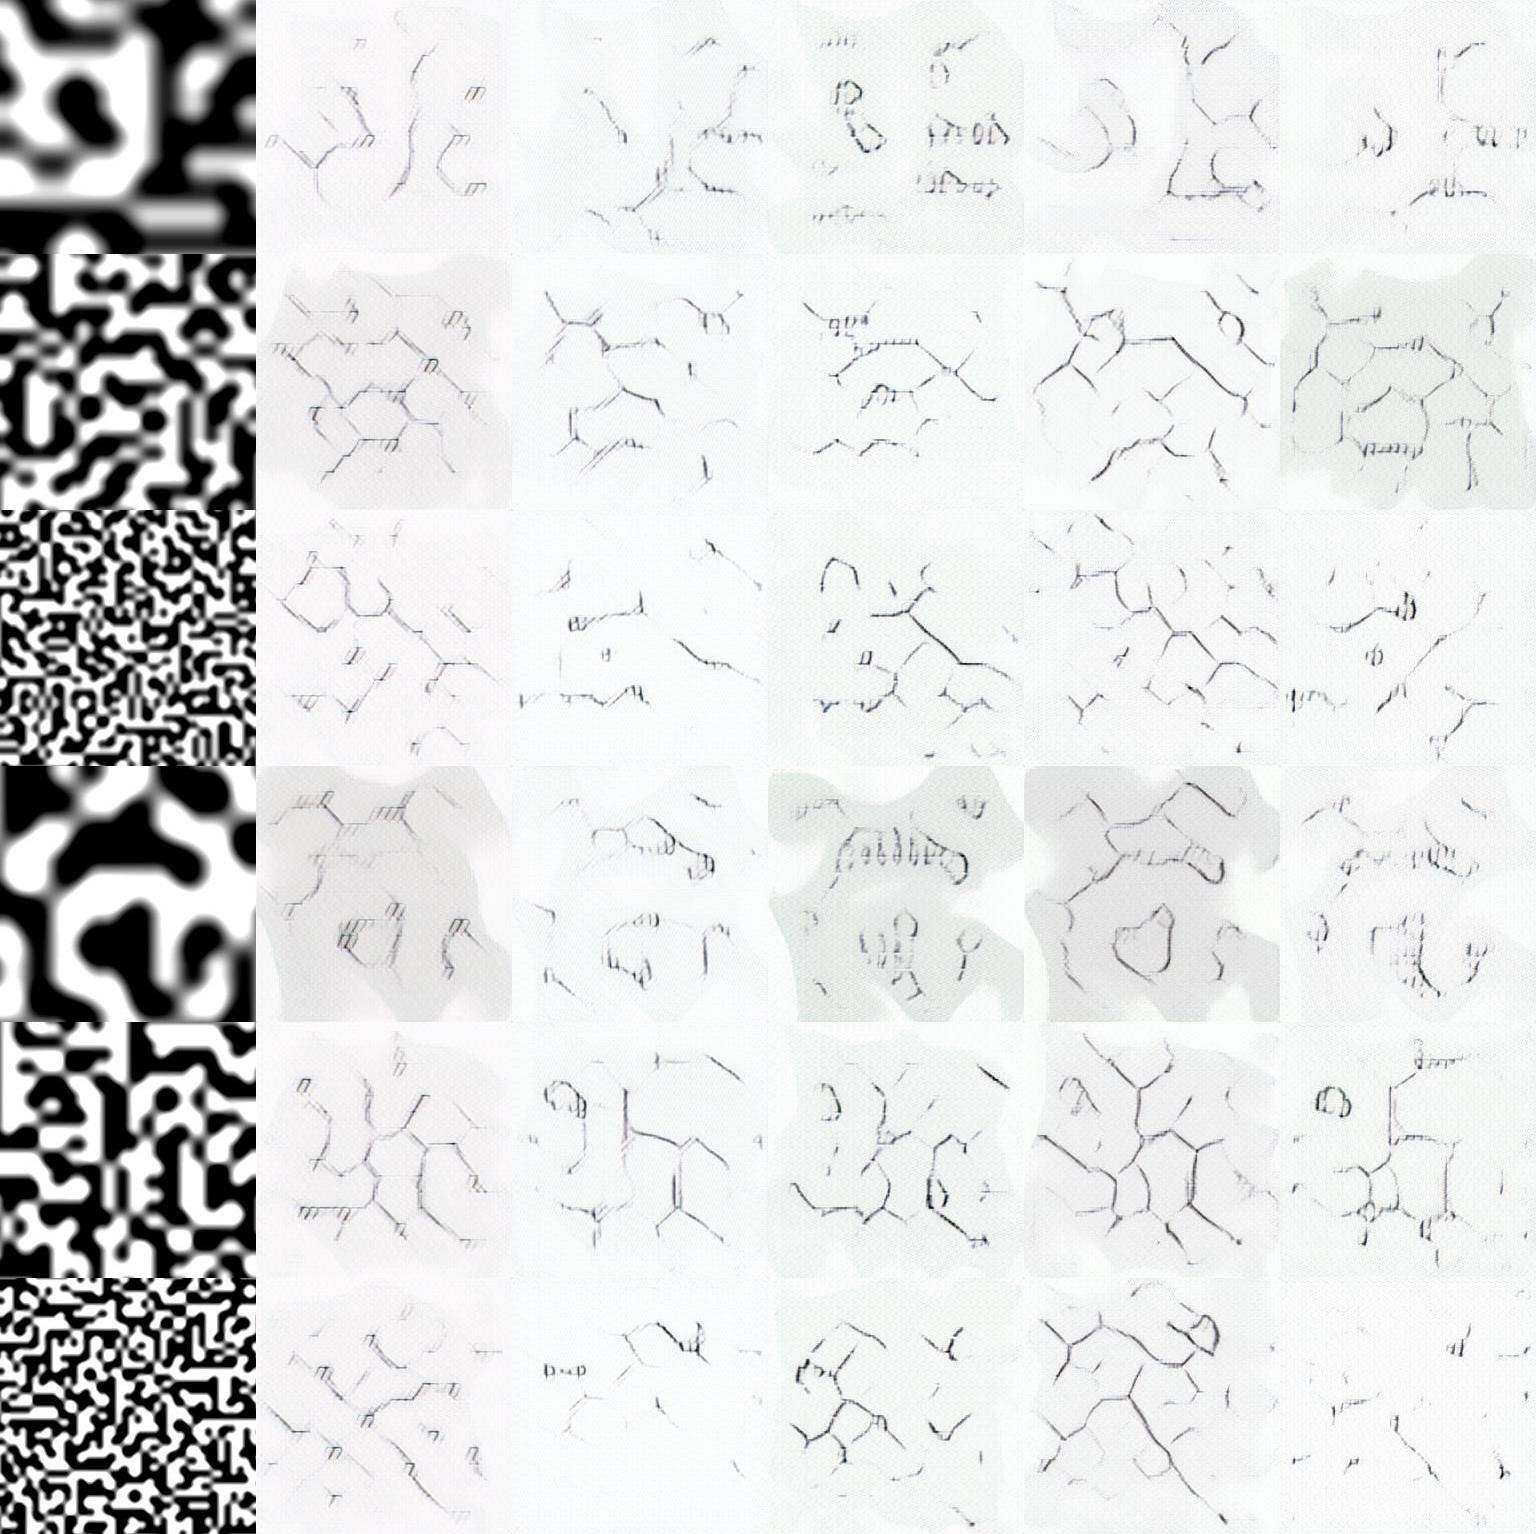
\includegraphics[scale=0.23]{imagenes/image_generation/256/aug2_extraepochs_2.jpg}}  
\end{figure}

\newpage
\section{Clasificación de imágenes}
El segundo objetivo de este proyecto consiste en clasificar aquellas imágenes que contienen estructuras de moléculas organometálicas de aquellas que no. Para ello, utilizamos la biblioteca Pytorch que nos permitirá implementar modelos de forma sencilla y definir sus hiperparámetros.

A priori no podemos conocer que modelo funcionará mejor para este problema, por lo que implementaremos varios y compararemos su rendimiento. Vamos a elegir un modelo de tamaño pequeño, otro de tamaño mediano y otro de tamaño grande y comparar cuál es el más adecuado:
\begin{itemize}
    \item \textbf{LeNet5:} Modelo propuesto por Yann LeCun en 1998 \cite{lecun1998gradient}, fue una de las primeras redes convolutivas de la historia. Se diseñó con el propósito de reconocer imágenes de dígitos numéricos, y tras compararse su rendimiento con otros modelos en uso, se demostró que los sobrepasaba. Esto atrajo a muchos investigadores a esta incipiente línea de investigación y sentó las bases para las arquitecturas del futuro.
    \item \textbf{AlexNet:} Propuesto por Alex Krizhevsky en 2012 \cite{krizhevsky2012imagenet}, consiguió mejorar por un alto porcentaje a la siguiente mejor solución en el concurso ImageNet Large Scale Visual Recognition Challenge. La ventaja de este modelo frente a otros fue su profundidad, que le permitía reconocer imágenes más complejas con mayor precisión. Esta conllevó un aumento del número de parámetros y del tiempo de entrenamiento, que fue contrarrestado por el uso de GPUs que permitían paralelizarlo. Para combatir el sobreajuste se utilizó \textit{dropout}, donde los enlaces entre neuronas se desconectaban con una determinada probabilidad durante cada iteración del entrenamiento.
    \item \textbf{VGG16:} Desarrollado por el Visual Geometry Group (de sus siglas procede el nombre del modelo) de la Universidad de Oxford \cite{https://doi.org/10.48550/arxiv.1409.1556}, fue el ganador del concurso ImageNet en su edición de 2014. Una de las características que le permitió mejorar frente a otros modelos fue el uso de \textit{kernels} convolutivos de pequeño tamaño (3x3). Se presentaron varias versiones del algoritmo, cada una con un número de capas diferente. La que nosotros utilizamos, VGG16, cuenta con 16 capas.
\end{itemize}

En un principio, cada uno de estos modelos se diseñó para trabajar con un tamaño de imágenes y de salida específicos, pero nosotros los adaptamos para funcionar sobre imágenes 256x256 y vectores \textit{one-hot}. Estos vectores se utilizan en problemas de clasificación, de forma que cada coordenada del vector representa una de las clases (en nuestro caso dos clases, imagen de molécula o no). Cada coordenada se conoce como \textit{logit}.

Tras la implementación con estos cambios, el número de parámetros se incrementa. Por ejemplo, LeNet5 contaba originalmente con 62006 parámetros al trabajar con imágenes 28x28 y un vector de salida de tamaño 10, pero tras los cambios cuenta con 7393806. Las versiones modificadas de AlexNet y VGG16 cuentan respectivamente con 58289538 y 153263298 parámetros.

Cada uno de estos modelos tiene diferentes hiperparámetros configurables: el tamaño del lote de entrenamiento (\textit{batch size}), el optimizador que modifica los parámetros en cada iteración, la inicialización de los pesos, etc. Algunos de estos producen mejores resultados que otros en determinados dominios y arquitecturas. Es imposible probar todos los valores posibles, por lo que seleccionamos algunos que creemos que pueden dar buenos resultados y comprobamos cuáles lo dan: esto es lo que se conoce como \textit{grid search}.

Vamos a trabajar con tres hiperparámetros. Aunque podríamos hacer pruebas con más, el número de modelos a entrenar crecería exponencialmente:
\begin{itemize}
    \item \textbf{Tasa de aprendizaje (\textit{Learning rate}):} Es probablemente el hiperparámetro más importante. Si le damos un valor demasiado bajo, los pesos del modelo variarán en muy poca medida en cada iteración y el error decrecerá muy lentamente. Si su valor es muy alto, es posible que el valor de los pesos y del error oscile y el algoritmo no converja. Es conveniente probar con diferentes posibilidades: en nuestro caso vamos a comprobar el rendimiento de los modelos tomando 0.5, 0.05, 0.005, 0.0005 y 0.00005 como posibles valores. \cite{berzal2018redes}
    \item \textbf{Inicialización de los pesos:} Las redes neuronales dependen en gran medida de la inicialización de los pesos. Si todas las neuronas se inicializasen con el mismo valor, el modelo no sería capaz de aprender nada, ya que la derivada del gradiente sería la misma para todas. Las que vamos a utilizar son: \cite{pytorch-doc}
    \begin{itemize}
        \item \textit{He:} utilizada por defecto en PyTorch en sus capas completamente conectadas y convolutivas, He (también conocida como Kaiming) genera valores aleatorios a partir de una distribución uniforme $\mathcal{U}(-bound, bound)$, donde $bound = gain * \sqrt{\frac{3}{fan\_in}}$. El parámetro $fan\_in$ depende de la entrada a la neurona. Por otro lado, en la inicialización por defecto de PyTorch $gain$ depende de $a = \sqrt{5}$.
        \item \textit{Xavier:} Los valores aleatorios son generados a partir de una distribución uniforme $\mathcal{U}(-a, a)$, donde $a = \sqrt{\frac{6}{fan\_in + fan\_out}}$. 
    \end{itemize}
    Una correcta inicialización de los pesos evita el problema de la evanescencia del gradiente (durante el entrenamiento, este se vuelve cada vez menor aproximándose a cero, de forma que los pesos no cambian) y el de explosión del gradiente (este toma valores cada vez mayores, de forma que los pesos cambian en gran medida y el algoritmo diverge).
    \item \textbf{Algoritmo de optimización:} Como muchos otros algoritmos de aprendizaje automático, los de aprendizaje profundo son problemas de optimización donde se intenta reducir el error de una función objetivo $f$ definida sobre un conjunto de datos de entrenamiento. Este proceso de optimización se realiza de forma numérica, una forma de hacerlo es a partir del cálculo del gradiente descendiente, un proceso costoso por tener que calcular en numerosas ocasiones el valor de la función $f$ y de su derivada. La elección del algoritmo de optimización es importante, ya que de él dependen la convergencia a una buena solución y el actualizar los pesos de forma eficiente: \cite{berzal2018redes}
    \begin{itemize}
        \item \textit{SGD:} En el entrenamiento de redes neuronales, el gradiente se calcula a partir de los datos de entrenamiento. Si estos datos no son un conjunto representativo de la distribución real porque contienen ruido, la estimación no será correcta. El gradiente se puede calcular a partir de todos los datos de entrenamiento (aprendizaje por lotes), a partir de un subconjunto (aprendizaje por minilotes) o a partir de una única muestra (aprendizaje online). Cuantos más datos utilicemos para calcular el gradiente, menor será el error cometido al estimarlo, pero como hemos mencionado, los datos siempre pueden contener ruido y por tanto no podemos asegurar que los resultados sean correctos. El gradiente descendiente estocástico (\textit{Stochastic Gradient Descent}, SGD) engloba el aprendizaje por minilotes y el online, y aunque pueda parecer lo contrario por utilizar menos muestras en el cómputo del gradiente, mejora los resultados al permitir al algoritmo escapar de puntos de silla. Además, es mucho más eficiente ya que solo tiene en cuenta un número limitado de datos.
        \item \textit{AdaDelta:} Es una extensión de AdaGrad (\textit{Adaptative Gradients}), un optimizador que dota a cada parámetro de una tasa de aprendizaje independiente y que va actualizando su valor durante la ejecución del algoritmo. AdaDelta resuelve el principal problema de Adagrad, la disminución prematura de las tasas de aprendizaje. Esto se debe a que Adagrad la calcula a partir del gradiente acumulado de todas las iteraciones, en cambio AdaDelta sólo utiliza las $n$ iteraciones anteriores.
        \item \textit{Adam:} Se podría considerar una extensión de AdaDelta en la que se utilizan momentos. En concreto, este algoritmo calcula la estimación del primer momento del gradiente (media) y del segundo momento (varianza). A partir de ellos se define la fórmula que da nombre a este algoritmo.
    \end{itemize}
\end{itemize}

En las ejecuciones que vamos a realizar, la función de coste que utilizamos es la función de entropía cruzada (\textit{Cross Entropy Loss}). Esta función integra la función de activación \textit{Softmax}, de forma que cada logit es transformado en un valor probabilístico entre 0 y 1. 


La función de entropía cruzada tratará de minimizar la distancia entre las probabilidades devueltas por el modelo y la probabilidad real. Tras el entrenamiento, cuando realicemos una predicción, la clase a la que pertenecerá la muestra será aquella que esté representada por el \textit{logit} con mayor probabilidad. \cite{crossentropyloss}

\begin{figure}[H]
\centering
    \fbox{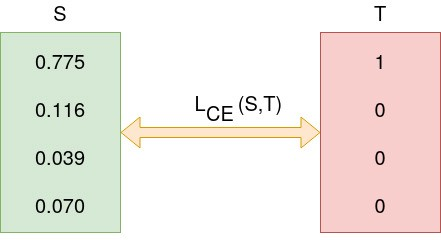
\includegraphics[scale=0.55]{imagenes/image_classification/crossentropyloss.jpeg}}
    \caption{La función de entropía cruzada $L_{CE}$ trata de minimizar la distancia entre el \textit{logit} $S$ y la etiqueta $T$ durante el entrenamiento. \cite{crossentropyloss}}
\end{figure}

Para la experimentación, dividimos el conjunto de datos en dos, train y test. Train tendrá el 85\% de las imágenes y test el 15\% restante. En la \textit{grid search} sólamente utilizaremos el conjunto train, sobre el que aplicaremos validación cruzada con 5 iteraciones. 

Finalmente, cuando hayamos decidido la configuración final, entrenaremos el modelo con el dataset de training al completo y evaluaremos su rendimiento con el de test.

El primer modelo con el que experimentamos es LeNet5. Los resultados obtenidos tras realizar la \textit{grid search} son los siguientes:

%TODO: Cambiar media por error medio (%) en el header de las tablas
\begin{table}[H]
\caption{\textit{Grid search} de los mejores parámetros sobre LeNet5}
\begin{tabular}{cl|llllll|}
\multicolumn{2}{c|}{\multirow{2}{*}{}}                                                                                                                              & \multicolumn{6}{c|}{Optimizadores}                                                                          \\ \cline{3-8} 
\multicolumn{2}{c|}{}                                                                                                                                               & \multicolumn{2}{c|}{SGD}             & \multicolumn{2}{c|}{Adam}            & \multicolumn{2}{c|}{AdaDelta} \\ \hline
\multicolumn{1}{c|}{\begin{tabular}[c]{@{}c@{}}Ini. de \\ pesos\end{tabular}} & \multicolumn{1}{c|}{\begin{tabular}[c]{@{}c@{}}Tasa de \\ aprendizaje\end{tabular}} & Media  & \multicolumn{1}{l|}{Desv.}  & Media  & \multicolumn{1}{l|}{Desv.}  & Media         & Desv.         \\ \hline
\multicolumn{1}{c|}{\multirow{5}{*}{He}}                                      & 0.5                                                                                 & 44.715 & \multicolumn{1}{l|}{1.971}  & 49.593 & \multicolumn{1}{l|}{6.630}  & 44.715        & 3.042         \\
\multicolumn{1}{c|}{}                                                         & 0.05                                                                                & 48.130 & \multicolumn{1}{l|}{6.308}  & 44.715 & \multicolumn{1}{l|}{3.042}  & 44.715        & 3.042         \\
\multicolumn{1}{c|}{}                                                         & 0.005                                                                               & 44.715 & \multicolumn{1}{l|}{3.042}  & 44.715 & \multicolumn{1}{l|}{3.042}  & 44.715        & 3.042         \\
\multicolumn{1}{c|}{}                                                         & 0.0005                                                                              & 44.715 & \multicolumn{1}{l|}{3.042}  & 44.715 & \multicolumn{1}{l|}{3.042}  & 44.715        & 3.042         \\
\multicolumn{1}{c|}{}                                                         & 0.00005                                                                             & 44.715 & \multicolumn{1}{l|}{3.042}  & 44.715 & \multicolumn{1}{l|}{3.042}  & 48.130        & 6.308         \\ \hline
\multicolumn{1}{c|}{\multirow{5}{*}{Xavier}}                                  & 0.5                                                                                 & 48.130 & \multicolumn{1}{l|}{6.308}  & 48.943 & \multicolumn{1}{l|}{6.540}  & 25.854        & 16.619        \\
\multicolumn{1}{c|}{}                                                         & 0.05                                                                                & 27.967 & \multicolumn{1}{l|}{14.734} & 44.715 & \multicolumn{1}{l|}{3.042}  & 33.252        & 11.226        \\
\multicolumn{1}{c|}{}                                                         & 0.005                                                                               & 43.902 & \multicolumn{1}{l|}{4.378}  & 44.715 & \multicolumn{1}{l|}{3.042}  & 43.740        & 4.685         \\
\multicolumn{1}{c|}{}                                                         & 0.0005                                                                              & 44.715 & \multicolumn{1}{l|}{3.042}  & 44.715 & \multicolumn{1}{l|}{3.042}  & 44.715        & 3.042         \\
\multicolumn{1}{c|}{}                                                         & 0.00005                                                                             & 44.715 & \multicolumn{1}{l|}{3.042}  & 39.756 & \multicolumn{1}{l|}{10.586} & 48.130        & 6.308        
\end{tabular}
\end{table}

Como se puede observar, el resultado es extraño: el modelo no parece estar aprendiendo nada. En ninguna de las configuraciones se observa que el error de clasificación sea bajo, y en aquellos casos donde se da esta situación Xavier con AdaDelta y tasa de aprendizaje 0.5 donde se consigue un 25\% de error, la desviación estándar entre iteraciones es del 16\%, una cifra alta. 





¿Por qué LeNet5 no está aprendiendo? Habiendo comprobado el modelo por si se tratase de un error de implementación y no habiendo encontrado ningún problema, vamos a probar a entrenarlo con una sola imagen, para comprobar si el error desciende en este caso.




% Please add the following required packages to your document preamble:
% \usepackage{multirow}
\begin{table}[H]
\caption{\textit{Grid search} de los mejores parámetros sobre AlexNet}
\begin{tabular}{cl|llllll|}
\multicolumn{2}{c|}{\multirow{2}{*}{}}                                                                                                                              & \multicolumn{6}{c|}{Optimizadores}                                                                              \\ \cline{3-8} 
\multicolumn{2}{c|}{}                                                                                                                                               & \multicolumn{2}{c|}{SGD}            & \multicolumn{2}{c|}{Adam}           & \multicolumn{2}{c|}{AdaDelta}       \\ \hline
\multicolumn{1}{c|}{\begin{tabular}[c]{@{}c@{}}Ini. de \\ pesos\end{tabular}} & \multicolumn{1}{c|}{\begin{tabular}[c]{@{}c@{}}Tasa de \\ aprendizaje\end{tabular}} & Media  & \multicolumn{1}{l|}{Desv.} & Media  & \multicolumn{1}{l|}{Desv.} & Media  & Desv.                      \\ \hline
\multicolumn{1}{c|}{\multirow{5}{*}{He}}                                      & 0.5                                                                                 & 44.715 & \multicolumn{1}{l|}{3.042} & 49.268 & \multicolumn{1}{l|}{7.061} & 5.041  & 1.691                      \\
\multicolumn{1}{c|}{}                                                         & 0.05                                                                                & 5.528  & \multicolumn{1}{l|}{1.809} & 53.008 & \multicolumn{1}{l|}{5.732} & 3.984  & 2.061                      \\
\multicolumn{1}{c|}{}                                                         & 0.005                                                                               & 3.984  & \multicolumn{1}{l|}{1.091} & 42.683 & \multicolumn{1}{l|}{6.814} & 5.366  & 1.449                      \\
\multicolumn{1}{c|}{}                                                         & 0.0005                                                                              & 44.634 & \multicolumn{1}{l|}{2.937} & 3.740  & \multicolumn{1}{l|}{1.128} & 44.715 & 3.042                      \\
\multicolumn{1}{c|}{}                                                         & 0.00005                                                                             & 44.715 & \multicolumn{1}{l|}{3.042} & 3.821  & \multicolumn{1}{r|}{0.843} & 45.691 & 2.104                      \\ \hline
\multicolumn{1}{c|}{\multirow{5}{*}{Xavier}}                                  & 0.5                                                                                 & 44.715 & \multicolumn{1}{l|}{3.042} & 46.992 & \multicolumn{1}{l|}{7.281} & 4.472  & \multicolumn{1}{r|}{0.909} \\
\multicolumn{1}{c|}{}                                                         & 0.05                                                                                & 5.691  & \multicolumn{1}{l|}{1.437} & 45.854 & \multicolumn{1}{l|}{7.113} & 3.984  & 1.661                      \\
\multicolumn{1}{c|}{}                                                         & 0.005                                                                               & 4.390  & \multicolumn{1}{l|}{1.937} & 44.634 & \multicolumn{1}{l|}{3.154} & 4.065  & 2.370                      \\
\multicolumn{1}{c|}{}                                                         & 0.0005                                                                              & 5.610  & \multicolumn{1}{l|}{2.360} & 4.146  & \multicolumn{1}{r|}{0.782} & 5.772  & 1.505                      \\
\multicolumn{1}{c|}{}                                                         & 0.00005                                                                             & 31.789 & \multicolumn{1}{l|}{2.325} & 3.333  & \multicolumn{1}{l|}{1.532} & 34.228 & 2.625                     
\end{tabular}
\end{table}

% Please add the following required packages to your document preamble:
% \usepackage{multirow}
\begin{table}[H]
\caption{\textit{Grid search} de los mejores parámetros sobre VGG16}
\begin{tabular}{cl|llllll|}
\multicolumn{2}{c|}{\multirow{2}{*}{}}                                                                                                                              & \multicolumn{6}{c|}{Optimizadores}                                                                                \\ \cline{3-8} 
\multicolumn{2}{c|}{}                                                                                                                                               & \multicolumn{2}{c|}{SGD}             & \multicolumn{2}{c|}{Adam}            & \multicolumn{2}{c|}{AdaDelta}       \\ \hline
\multicolumn{1}{c|}{\begin{tabular}[c]{@{}c@{}}Ini. de \\ pesos\end{tabular}} & \multicolumn{1}{c|}{\begin{tabular}[c]{@{}c@{}}Tasa de \\ aprendizaje\end{tabular}} & Media  & \multicolumn{1}{l|}{Desv.}  & Media  & \multicolumn{1}{l|}{Desv.}  & Media  & Desv.                      \\ \hline
\multicolumn{1}{c|}{\multirow{5}{*}{He}}                                      & 0.5                                                                                 & 44.715 & \multicolumn{1}{l|}{3.042}  & 52.439 & \multicolumn{1}{l|}{5.126}  & 44.715 & 3.042                      \\
\multicolumn{1}{c|}{}                                                         & 0.05                                                                                & 44.715 & \multicolumn{1}{l|}{3.042}  & 45.122 & \multicolumn{1}{l|}{2.787}  & 44.715 & 3.042                      \\
\multicolumn{1}{c|}{}                                                         & 0.005                                                                               & 44.715 & \multicolumn{1}{l|}{3.042}  & 44.715 & \multicolumn{1}{l|}{3.042}  & 44.715 & 3.042                      \\
\multicolumn{1}{c|}{}                                                         & 0.0005                                                                              & 44.715 & \multicolumn{1}{l|}{3.042}  & 37.967 & \multicolumn{1}{l|}{17.082} & 48.537 & 7.062                      \\
\multicolumn{1}{c|}{}                                                         & 0.00005                                                                             & 48.618 & \multicolumn{1}{l|}{6.938}  & 5.041  & \multicolumn{1}{r|}{1.171}  & 50.569 & 5.436                      \\ \hline
\multicolumn{1}{c|}{\multirow{5}{*}{Xavier}}                                  & 0.5                                                                                 & 44.715 & \multicolumn{1}{l|}{3.042}  & 49.350 & \multicolumn{1}{l|}{6.463}  & 44.715 & \multicolumn{1}{r|}{3.042} \\
\multicolumn{1}{c|}{}                                                         & 0.05                                                                                & 18.049 & \multicolumn{1}{l|}{15.009} & 44.715 & \multicolumn{1}{l|}{3.042}  & 3.333  & 1.758                      \\
\multicolumn{1}{c|}{}                                                         & 0.005                                                                               & 8.618  & \multicolumn{1}{l|}{7.142}  & 44.715 & \multicolumn{1}{l|}{3.042}  & 7.154  & 1.786                      \\
\multicolumn{1}{c|}{}                                                         & 0.0005                                                                              & 44.309 & \multicolumn{1}{l|}{3.613}  & 44.715 & \multicolumn{1}{r|}{3.042}  & 44.472 & 3.562                      \\
\multicolumn{1}{c|}{}                                                         & 0.00005                                                                             & 46.260 & \multicolumn{1}{l|}{2.139}  & 2.846  & \multicolumn{1}{r|}{0.996}  & 48.130 & 4.010                     
\end{tabular}
\end{table}